% resultados_v2_completo.tex: whole Overleaf package in one file (body of the document, after \begin{document}).
% Generated by 02_scripts/12_paquete_overleaf.py.
% Packages needed in the preamble of main.tex: graphicx, caption, subcaption, booktabs, longtable, float, pdflscape.
% Figures: \graphicspath{{figuras/}{figures/}} in main.tex; \includegraphics uses only the file name.
% Fill in the MIDAGRI-SISAGRI access date once, in \midagridate below.

% ===== captions.tex =====
% Figure captions, taken from the .txt file of each figure (08_graficos/) with internal references removed.
% Generated by 02_scripts/12_paquete_overleaf.py.
% Date of access to MIDAGRI-SISAGRI: fill in ONCE here; it is used by every caption and by Table S1.
\newcommand{\midagridate}{[____]}

% One \newcommand per figure, named after the figure file: \figcap{<file name>} prints its caption.
\newcommand{\defcap}[2]{\expandafter\newcommand\csname figcap-#1\endcsname{#2}}
\newcommand{\figcap}[1]{\ifcsname figcap-#1\endcsname\csname figcap-#1\endcsname\else\PackageError{captions}{No caption for #1}{}\fi}

\defcap{fig29_study_area_map}{Lime-producing provinces of Peru and their cumulative production, January 2016–December 2025: (a) sour lime, (b) sweet lime (MIDAGRI–SISAGRI (accessed \midagridate{})). Circle area is proportional to each province's cumulative production of that cultivar; labels give the five largest provinces and their share of the national total of that cultivar. Symbols show whether a province recorded sour lime only, both cultivars, sweet lime only or no harvest in the period (109 provinces). Dashed rings: ten provinces placed at their department's reference coordinate, including the two sweet-lime-only and the four no-harvest provinces. Boundaries: geoBoundaries gbOpen (Runfola et al., 2020), Public Domain, 2008 vintage; neighbouring countries: Natural Earth 1:10m.}
\defcap{fig24_series_with_shocks_sutil}{Monthly national production of sour lime (limón sutil) in Peru, January 2016–December 2025 (MIDAGRI–SISAGRI (accessed \midagridate{})). Grey bands and markers: shock months in the test years 2021–2025, i.e. months whose absolute month-on-month relative change \textbar{}$\Delta$y/y\textbar{} exceeds the 75th percentile of the changes observed up to the forecast origin (December of the previous year); the threshold of each test year is shown above the panel. No month exceeded the threshold in 2021 or 2024.}
\defcap{fig24_series_with_shocks_dulce}{Monthly national production of sweet lime (limón dulce) in Peru, January 2016–December 2025 (MIDAGRI–SISAGRI (accessed \midagridate{})). Grey bands and markers: shock months in the test years 2021–2025, i.e. months whose absolute month-on-month relative change \textbar{}$\Delta$y/y\textbar{} exceeds the 75th percentile of the changes observed up to the forecast origin (December of the previous year); the threshold of each test year is shown above the panel. 14 of the 15 shock months fall in January–March.}
\defcap{fig_workflow}{Study workflow. (1) Monthly data, 2016–2025: national lime production (MIDAGRI–SISAGRI (accessed \midagridate{})), NASA POWER climate, INDECI disaster records and agricultural news from Agraria.pe, scored with the pysentimiento RoBERTuito sentiment model (monthly mean sentiment and number of news items). (2) In each window, predictors enter with lags 1, 3 and 6 months; the scaler and the geographic weights are fitted on the training data only (up to December of Y\textminus{}2), and the shock threshold is computed with the history up to the forecast origin (December of Y\textminus{}1). (3) Rolling-origin evaluation with the origin in December of Y\textminus{}1: training up to December of Y\textminus{}2, validation in year Y\textminus{}1 and test in year Y, for test years 2018–2025. In 2018–2020 only Naive, Seasonal Naive and Chronos are run (trained models need at least 36 training months). The model ranking uses 2021–2025; 2023–2025 is a pre-registered sensitivity set. (4) 10 models: Naive, Seasonal Naive, Chronos, SARIMA, SARIMA-sel, Ridge, ElasticNet, XGB-37, GC3 and GE. XGB-37, GC3 and GE are run with 10 seeds (0–9), and their monthly absolute errors are averaged over seeds. XGB-43 (dashed) is an exploratory, post hoc model outside the ranking. (5) MAE over all, shock and normal months; $\Delta$s = (MAE\_shock \textminus{} MAE)/MAE × 100; paired bootstrap 95\% confidence intervals (months resampled within windows, B = 10,000); Diebold–Mariano tests with the Harvey–Leybourne–Newbold correction. The Holm adjustment is exploratory. Shock month (main definition): month-on-month change \textbar{}y\_t \textminus{} y\_(t\textminus{}1)\textbar{}/y\_(t\textminus{}1) above the 75th percentile of the changes observed up to the forecast origin; the 50th, 60th and 90th percentiles and the year-on-year change are reported as sensitivity. No results are shown in this figure.}
\defcap{fig30_rolling_origin_scheme}{Rolling-origin evaluation design. For each test year Y (2018–2025) the forecast origin is December of Y\textminus{}1; trained models use data up to December of Y\textminus{}2 (features from 2016-07; tabular targets from 2016-08; LSTM targets from 2017-01), are tuned and early-stopped on year Y\textminus{}1, and produce twelve one-step-ahead forecasts for year Y. Trained models require at least 36 training months, so windows 2018–2020 (faded) include only the untrained models (Naive, Seasonal Naive, Chronos). The primary ranking pools the windows 2021–2025; a pre-registered sensitivity analysis repeats all conclusions on 2023–2025.}
\defcap{fig25_architecture_dual_lstm}{Dual-LSTM with additive (Bahdanau) temporal attention used by GC3 and GE. Each branch receives the previous 6 months: branch A the production series and its lags 1, 3 and 6; branch B calendar terms, a time index and lagged climate (NASA POWER) and disaster (INDECI) covariates. GE adds six lagged news features to branch B (dashed box): the monthly mean sentiment score of agricultural news, computed with the pysentimiento RoBERTuito sentiment model, and the monthly number of news items. GC3 and GE are otherwise identical. Trainable parameters: GC3 6,273; GE 6,657.}
\defcap{fig13_mae_normal_vs_shock_bars_sutil}{MAE in normal months (light) and in shock months (hatched; monthly P75 threshold) for each model, sour lime (limón sutil), pooled 2021–2025, with paired bootstrap 95\% CIs.}
\defcap{fig13_mae_normal_vs_shock_bars_dulce}{MAE in normal months (light) and in shock months (hatched; monthly P75 threshold) for each model, sweet lime (limón dulce), pooled 2021–2025, with paired bootstrap 95\% CIs.}
\defcap{fig07_rank_heatmap_model_percentile_sutil}{Rank of each model by MAE\_shock at every threshold percentile (P0–P95), sour lime (limón sutil), 2021–2025: (a) month-on-month and (b) year-on-year change. Numbers are ranks; * marks the first place and statistical ties with it.}
\defcap{fig07_rank_heatmap_model_percentile_dulce}{Rank of each model by MAE\_shock at every threshold percentile (P0–P95), sweet lime (limón dulce), 2021–2025: (a) month-on-month and (b) year-on-year change. Numbers are ranks; * marks the first place and statistical ties with it.}
\defcap{fig05_mae_shock_vs_percentile_sutil}{Mean absolute error in shock months (tonnes) versus shock-threshold percentile, sour lime (limón sutil), 2021–2025 pooled. Errors of seeded models are averaged over 10 seeds per month (pre-registered). Dashed lines: P50, P60, P75, P90.}
\defcap{fig05_mae_shock_vs_percentile_dulce}{Mean absolute error in shock months (tonnes) versus shock-threshold percentile, sweet lime (limón dulce), 2021–2025 pooled. Errors of seeded models are averaged over 10 seeds per month (pre-registered). Dashed lines: P50, P60, P75, P90. Logarithmic y-axis.}
\defcap{fig04_delta_s_vs_percentile_sutil}{Relative shock penalty $\Delta$s versus shock-threshold percentile (P0–P95), sour lime (limón sutil), pooled test windows 2021–2025. Dashed lines mark the reporting points P50, P60, P75 (primary) and P90.}
\defcap{fig04_delta_s_vs_percentile_dulce}{Relative shock penalty $\Delta$s versus shock-threshold percentile (P0–P95), sweet lime (limón dulce), pooled test windows 2021–2025. Dashed lines mark the reporting points P50, P60, P75 (primary) and P90.}
\defcap{fig10_n_shock_heatmap_window_percentile_sutil}{Shock months per test window and threshold percentile, sour lime (limón sutil): (a) month-on-month, (b) year-on-year. Thresholds are computed with the history up to each origin. \dag{} = fewer than 2 shocks (non-informative window).}
\defcap{fig10_n_shock_heatmap_window_percentile_dulce}{Shock months per test window and threshold percentile, sweet lime (limón dulce): (a) month-on-month, (b) year-on-year. Thresholds are computed with the history up to each origin. \dag{} = fewer than 2 shocks (non-informative window).}
\defcap{fig20_real_vs_pred_2025_sutil}{Observed national production and one-step-ahead forecasts of each model, test year 2025, sour lime (limón sutil). Grey: shock months (monthly P75, history to origin). Seeded models: one line per seed (10 seeds). Observed: thick black line; Seasonal Naive: dashed black line with open squares.}
\defcap{fig20_real_vs_pred_2025_dulce}{Observed national production and one-step-ahead forecasts of each model, test year 2025, sweet lime (limón dulce). Grey: shock months (monthly P75, history to origin). Seeded models: one line per seed (10 seeds). Observed: thick black line; Seasonal Naive: dashed black line with open squares.}
\defcap{fig18_nlp_ablation_paired_sutil}{NLP ablation: difference in MAE between GE (Dual-LSTM with NLP features) and GC3 (same architecture without NLP), paired by seed, sour lime (limón sutil), per test window and pooled; (a) all months, (b) shock months (monthly P75), (c) normal months. Dots: individual seed pairs; diamonds: mean with paired bootstrap 95\% CI (months resampled within windows, B = 10,000). n/a = no shock month.}
\defcap{fig18_nlp_ablation_paired_dulce}{NLP ablation: difference in MAE between GE (Dual-LSTM with NLP features) and GC3 (same architecture without NLP), paired by seed, sweet lime (limón dulce), per test window and pooled; (a) all months, (b) shock months (monthly P75), (c) normal months. Dots: individual seed pairs; diamonds: mean with paired bootstrap 95\% CI (months resampled within windows, B = 10,000). n/a = no shock month.}
\defcap{fig02_train_val_gap_sutil}{Validation/training MAE ratio for each trained model, window and seed (points), sour lime (limón sutil); grey bars: same ratio for the Naive forecast on the training and validation months of the tabular models (on the LSTM months, which start in 2017-01, it differs by at most 0.030); dashed line: overfitting flag at 2.0 (pre-registered). In Sutil the validation year has a higher mean level than the training period in 2021, 2022, 2023, 2025, which inflates the ratio.}
\defcap{fig02_train_val_gap_dulce}{Validation/training MAE ratio for each trained model, window and seed (points), sweet lime (limón dulce); grey bars: same ratio for the Naive forecast on the training and validation months of the tabular models (on the LSTM months, which start in 2017-01, it differs by at most 0.015); dashed line: overfitting flag at 2.0 (pre-registered).}
\defcap{fig20_real_vs_pred_2023_sutil}{Observed national production and one-step-ahead forecasts of each model, test year 2023, sour lime (limón sutil). Grey: shock months (monthly P75, history to origin). Seeded models: one line per seed (10 seeds). Observed: thick black line; Seasonal Naive: dashed black line with open squares.}
\defcap{fig20_real_vs_pred_2024_dulce}{Observed national production and one-step-ahead forecasts of each model, test year 2024, sweet lime (limón dulce). Grey: shock months (monthly P75, history to origin). Seeded models: one line per seed (10 seeds). Observed: thick black line; Seasonal Naive: dashed black line with open squares.}
\defcap{fig19_dm_pvalue_matrix_sutil}{Diebold–Mariano tests with the Harvey–Leybourne–Newbold correction (h = 1, absolute loss, seed-averaged errors, pooled windows 2021–2025), sour lime (limón sutil): unadjusted p-values. Lower triangle: all test months (n = 60); upper triangle: shock months only (monthly P75, n = 10). '+' = row model has larger error than column model.}
\defcap{fig19_dm_pvalue_matrix_dulce}{Diebold–Mariano tests with the Harvey–Leybourne–Newbold correction (h = 1, absolute loss, seed-averaged errors, pooled windows 2021–2025), sweet lime (limón dulce): unadjusted p-values. Lower triangle: all test months (n = 60); upper triangle: shock months only (monthly P75, n = 15). '+' = row model has larger error than column model.}
\defcap{fig19b_dm_pvalue_matrix_holm_sutil}{Diebold–Mariano tests with the Harvey–Leybourne–Newbold correction (h = 1, absolute loss, seed-averaged errors, pooled windows 2021–2025), sour lime (limón sutil): Holm-adjusted (exploratory; family = 45 pairs per triangle) p-values. Lower triangle: all test months (n = 60); upper triangle: shock months only (monthly P75, n = 10). '+' = row model has larger error than column model. Holm correction is an exploratory addition, not part of the pre-registration.}
\defcap{fig19b_dm_pvalue_matrix_holm_dulce}{Diebold–Mariano tests with the Harvey–Leybourne–Newbold correction (h = 1, absolute loss, seed-averaged errors, pooled windows 2021–2025), sweet lime (limón dulce): Holm-adjusted (exploratory; family = 45 pairs per triangle) p-values. Lower triangle: all test months (n = 60); upper triangle: shock months only (monthly P75, n = 15). '+' = row model has larger error than column model. Holm correction is an exploratory addition, not part of the pre-registration.}
\defcap{fig18b_xgb43_vs_xgb37_exploratory_sutil}{EXPLORATORY (post-hoc) comparison: difference in MAE between XGB-43 and XGB-37, paired by seed, sour lime (limón sutil); (a) all months, (b) shock months (monthly P75, MoM), (c) normal months. XGB-43 uses the 37 predictors of XGB-37 plus six lagged NLP features (avg\_sentiment and n\_noticias at lags 1, 3 and 6) with the same hyperparameters. Dots: individual seed pairs per test window (2021–2025) and pooled 2021–2025; diamond: mean over 10 seeds for the pooled 2021–2025 set with paired bootstrap 95\% CI (months resampled within windows, B = 10,000). No mean or CI is shown per window. n/a = no shock month. XGB-43 was added post hoc: it is not part of the preregistered ranking and is not included in the Diebold–Mariano tests or the Holm correction.}
\defcap{fig18b_xgb43_vs_xgb37_exploratory_dulce}{EXPLORATORY (post-hoc) comparison: difference in MAE between XGB-43 and XGB-37, paired by seed, sweet lime (limón dulce); (a) all months, (b) shock months (monthly P75, MoM), (c) normal months. XGB-43 uses the 37 predictors of XGB-37 plus six lagged NLP features (avg\_sentiment and n\_noticias at lags 1, 3 and 6) with the same hyperparameters. Dots: individual seed pairs per test window (2021–2025) and pooled 2021–2025; diamond: mean over 10 seeds for the pooled 2021–2025 set with paired bootstrap 95\% CI (months resampled within windows, B = 10,000). No mean or CI is shown per window. n/a = no shock month. XGB-43 was added post hoc: it is not part of the preregistered ranking and is not included in the Diebold–Mariano tests or the Holm correction.}
\defcap{fig01_loss_curves_gc3_sutil}{Training and validation loss curves of GC3 for each test window and the 10 seeds (one line per seed), sour lime (limón sutil). Dots: epoch with minimum validation loss, whose weights are restored for forecasting.}
\defcap{fig01_loss_curves_gc3_dulce}{Training and validation loss curves of GC3 for each test window and the 10 seeds (one line per seed), sweet lime (limón dulce). Dots: epoch with minimum validation loss, whose weights are restored for forecasting.}
\defcap{fig01_loss_curves_ge_sutil}{Training and validation loss curves of GE for each test window and the 10 seeds (one line per seed), sour lime (limón sutil). Dots: epoch with minimum validation loss, whose weights are restored for forecasting.}
\defcap{fig01_loss_curves_ge_dulce}{Training and validation loss curves of GE for each test window and the 10 seeds (one line per seed), sweet lime (limón dulce). Dots: epoch with minimum validation loss, whose weights are restored for forecasting.}
\defcap{fig03_early_stopping_epoch_sutil}{Distribution over 10 seeds of the best (restored) epoch of GC3 and GE per test window, sour lime (limón sutil); early stopping on validation year Y\textminus{}1, patience 15, maximum 300 epochs.}
\defcap{fig03_early_stopping_epoch_dulce}{Distribution over 10 seeds of the best (restored) epoch of GC3 and GE per test window, sweet lime (limón dulce); early stopping on validation year Y\textminus{}1, patience 15, maximum 300 epochs.}
\defcap{fig06_ratio_shock_normal_vs_percentile_sutil}{Ratio of shock-month to normal-month MAE versus threshold percentile, sour lime (limón sutil), 2021–2025. Undefined at P0. Horizontal line: ratio = 1. Logarithmic y-axis, so ratios r and 1/r are equally far from 1.}
\defcap{fig06_ratio_shock_normal_vs_percentile_dulce}{Ratio of shock-month to normal-month MAE versus threshold percentile, sweet lime (limón dulce), 2021–2025. Undefined at P0. Horizontal line: ratio = 1. Logarithmic y-axis, so ratios r and 1/r are equally far from 1.}
\defcap{fig08_rank_bump_chart_sutil}{Rank trajectories by MAE\_shock across monthly threshold percentiles, sour lime (limón sutil), 2021–2025. Open circles: first place or tied with it (paired bootstrap). Dashed lines: P50, P60, P75, P90.}
\defcap{fig08_rank_bump_chart_dulce}{Rank trajectories by MAE\_shock across monthly threshold percentiles, sweet lime (limón dulce), 2021–2025. Open circles: first place or tied with it (paired bootstrap). Dashed lines: P50, P60, P75, P90.}
\defcap{fig09_n_shock_vs_percentile_sutil}{Number of shock months in the pooled 2021–2025 test set versus threshold percentile, sour lime (limón sutil); solid: month-on-month change, dashed: year-on-year change.}
\defcap{fig09_n_shock_vs_percentile_dulce}{Number of shock months in the pooled 2021–2025 test set versus threshold percentile, sweet lime (limón dulce); solid: month-on-month change, dashed: year-on-year change.}
\defcap{fig11_bootstrap_ci_mae_shock_report_points_sutil}{MAE in shock months with paired bootstrap 95\% confidence intervals (i.i.d. over months, stratified by window, B = 10,000) at the reporting thresholds P50, P60, P75 and P90 (monthly), sour lime (limón sutil), 2021–2025.}
\defcap{fig11_bootstrap_ci_mae_shock_report_points_dulce}{MAE in shock months with paired bootstrap 95\% confidence intervals (i.i.d. over months, stratified by window, B = 10,000) at the reporting thresholds P50, P60, P75 and P90 (monthly), sweet lime (limón dulce), 2021–2025. Logarithmic x-axis.}
\defcap{fig12_yoy_vs_mom_threshold_sutil}{MAE in shock months versus threshold percentile for each model, month-on-month (solid) versus year-on-year (dashed) shock definition, sour lime (limón sutil), 2021–2025. Each panel has its own y-axis.}
\defcap{fig12_yoy_vs_mom_threshold_dulce}{MAE in shock months versus threshold percentile for each model, month-on-month (solid) versus year-on-year (dashed) shock definition, sweet lime (limón dulce), 2021–2025. Each panel has its own y-axis.}
\defcap{fig14_mae_shock_heatmap_model_window_sutil}{MAE in shock months (monthly P75) by model and test window, sour lime (limón sutil). n/a = no shock month in that window.}
\defcap{fig14_mae_shock_heatmap_model_window_dulce}{MAE in shock months (monthly P75) by model and test window, sweet lime (limón dulce). n/a = no shock month in that window.}
\defcap{fig15_seed_boxplots_sutil}{Distribution over the 10 training seeds of (a) MAE and (b) shock-month MAE (monthly P75) per test window and pooled 2021–2025, for the seeded models, sour lime (limón sutil).}
\defcap{fig15_seed_boxplots_dulce}{Distribution over the 10 training seeds of (a) MAE and (b) shock-month MAE (monthly P75) per test window and pooled 2021–2025, for the seeded models, sweet lime (limón dulce).}
\defcap{fig16_mae_by_change_quartile_sutil}{MAE by quartile of the absolute month-on-month relative change \textbar{}$\Delta$y/y\textbar{} of the test months, sour lime (limón sutil), pooled 2021–2025.}
\defcap{fig16_mae_by_change_quartile_dulce}{MAE by quartile of the absolute month-on-month relative change \textbar{}$\Delta$y/y\textbar{} of the test months, sweet lime (limón dulce), pooled 2021–2025.}
\defcap{fig17_leave_one_shock_out_delta_s_sutil}{$\Delta$s with all shock months (marker) and its range when one shock month is removed at a time (bar), sour lime (limón sutil), pooled 2021–2025, monthly P75.}
\defcap{fig17_leave_one_shock_out_delta_s_dulce}{$\Delta$s with all shock months (marker) and its range when one shock month is removed at a time (bar), sweet lime (limón dulce), pooled 2021–2025, monthly P75.}
\defcap{fig21_abs_error_monthly_sutil}{Month-by-month absolute forecast error of each model (mean over seeds for seeded models), sour lime (limón sutil), test months 2021–2025.}
\defcap{fig21_abs_error_monthly_dulce}{Month-by-month absolute forecast error of each model (mean over seeds for seeded models), sweet lime (limón dulce), test months 2021–2025.}

% ===== tables_main.tex =====
% Tables, main text, in order of appearance (generated from the CSV files of 06_metricas/).

% --- tables/TM1_descriptive_series.tex
\begin{table}[htbp]
\centering
\small
\caption{Descriptive statistics of the national monthly production series for each rolling-origin window, 2021--2025. Mean, standard deviation (SD) and coefficient of variation (CV) refer to the 12 months of the test year. Train months, autocorrelation (ACF at lags 1 and 12) and unit-root tests refer to the training partition of each window, series in levels with a constant: ADF (null hypothesis: unit root) and KPSS (null hypothesis: level stationarity) $p$-values; KPSS $p$-values outside the tabulated range are shown as bounds.}
\label{tab:main_descriptive_series}
\begin{tabular}{lrrrrrrrr}
\toprule
Test year & Train months & Mean (t) & SD (t) & CV & ACF(1) & ACF(12) & ADF $p$ & KPSS $p$ \\
\midrule
\multicolumn{9}{l}{\textit{Sour lime}} \\
2021 & 42 & 27,980 & 4,362 & 0.16 & 0.84 & 0.33 & 0.011 & $>$0.10 \\
2022 & 54 & 30,558 & 8,004 & 0.26 & 0.81 & 0.49 & 0.004 & $>$0.10 \\
2023 & 66 & 23,067 & 8,319 & 0.36 & 0.84 & 0.55 & 0.002 & 0.035 \\
2024 & 78 & 32,209 & 8,550 & 0.27 & 0.86 & 0.56 & 0.863 & 0.016 \\
2025 & 90 & 31,908 & 9,103 & 0.29 & 0.85 & 0.58 & 0.641 & 0.039 \\
\addlinespace
\multicolumn{9}{l}{\textit{Sweet lime}} \\
2021 & 42 & 393.8 & 144.0 & 0.37 & 0.79 & 0.67 & 0.267 & $>$0.10 \\
2022 & 54 & 406.4 & 154.5 & 0.38 & 0.80 & 0.74 & 0.915 & $>$0.10 \\
2023 & 66 & 406.5 & 159.9 & 0.39 & 0.81 & 0.79 & 0.779 & $>$0.10 \\
2024 & 78 & 448.3 & 161.4 & 0.36 & 0.81 & 0.81 & 0.446 & $>$0.10 \\
2025 & 90 & 467.8 & 177.3 & 0.38 & 0.82 & 0.83 & 0.377 & $>$0.10 \\
\bottomrule
\end{tabular}
\end{table}

% --- tables/TM2_aggregate_accuracy_P75.tex
\begin{table}[htbp]
\centering
\small
\caption{Aggregated forecast accuracy, pooled test windows 2021--2025, by cultivar. Shock months: monthly P75 threshold of the month-on-month change (history up to each origin). MAE in tonnes with 95\% bootstrap confidence intervals in parentheses (months resampled within windows, B = 10,000); $\Delta_s = (\mathrm{MAE}_{\mathrm{shock}} - \mathrm{MAE})/\mathrm{MAE} \times 100$. Errors of seeded models (XGB-37, GC3, GE) are averaged over 10 seeds per month. The exploratory XGB-43 is not included.}
\label{tab:main_aggregate_accuracy}
\begin{tabular}{lccr}
\toprule
Model & MAE, all months (t) (95\% CI) & MAE, shock months (t) (95\% CI) & $\Delta_s$ (\%) \\
\midrule
\multicolumn{4}{l}{\textit{Sour lime} (60 test months; 10 shock months)} \\
Naive & 3,624 (2,920--4,382) & 8,506 (7,724--9,215) & 134.7 \\
Seasonal Naive & 6,075 (5,156--6,987) & 5,034 (2,259--7,928) & -17.1 \\
Chronos & 2,649 (2,171--3,144) & 4,784 (3,963--5,641) & 80.6 \\
SARIMA & 3,361 (2,780--3,970) & 5,131 (3,759--6,624) & 52.7 \\
SARIMA-sel & 3,206 (2,563--3,880) & 4,936 (2,866--7,242) & 54.0 \\
Ridge & 4,925 (3,838--6,074) & 8,557 (5,484--12,360) & 73.7 \\
ElasticNet & 4,872 (3,847--5,950) & 8,154 (5,162--11,484) & 67.4 \\
XGB-37 & 4,881 (4,063--5,732) & 5,955 (3,727--7,965) & 22.0 \\
GC3 & 6,361 (5,292--7,446) & 6,074 (4,085--8,216) & -4.5 \\
GE & 6,744 (5,587--7,894) & 6,827 (4,477--9,213) & 1.2 \\
\addlinespace
\multicolumn{4}{l}{\textit{Sweet lime} (60 test months; 15 shock months)} \\
Naive & 77.5 (65.7--89.9) & 131.6 (116.5--147.7) & 69.8 \\
Seasonal Naive & 24.5 (20.5--29.0) & 24.5 (21.4--27.8) & -0.0 \\
Chronos & 30.8 (25.6--36.4) & 48.2 (40.5--56.1) & 56.4 \\
SARIMA & 18.4 (14.5--22.8) & 14.0 (9.8--18.0) & -24.1 \\
SARIMA-sel & 20.6 (16.5--25.2) & 19.7 (15.6--23.6) & -4.5 \\
Ridge & 53.1 (43.4--63.4) & 69.7 (52.0--89.3) & 31.3 \\
ElasticNet & 50.2 (40.7--60.4) & 67.2 (49.5--87.1) & 33.8 \\
XGB-37 & 48.3 (39.8--57.2) & 65.8 (51.6--80.6) & 36.4 \\
GC3 & 56.7 (46.9--66.9) & 60.7 (46.2--76.3) & 7.2 \\
GE & 56.7 (47.5--66.7) & 57.9 (41.8--75.2) & 2.0 \\
\bottomrule
\end{tabular}
\end{table}

% --- tables/TM3_robust_ranking.tex
\begin{table}[htbp]
\centering
\small
\caption{Rank of each model by MAE in shock months, pooled test windows 2021--2025, at the reporting thresholds P50, P60, P75 and P90 of the month-on-month (MoM) change. $^{*}$ = first or statistically tied with the first (the 95\% paired bootstrap CI of the difference in MAE with the best model contains 0). A model is robust if it is first or tied in at least 3 of the 4 thresholds; the year-on-year (YoY) definition is evaluated separately and its ranks are not shown.}
\label{tab:main_robust_ranking}
\begin{tabular}{lccccrcrc}
\toprule
Model & P50 & P60 & P75 & P90 & First or tied, MoM (of 4) & Robust, MoM & First or tied, YoY (of 4) & Robust, YoY \\
\midrule
\multicolumn{9}{l}{\textit{Sour lime}} \\
Naive & 5 & 8 & 9 & 7 & 0 & No & 4 & Yes \\
Seasonal Naive & 6 & 5 & 3$^{*}$ & 4$^{*}$ & 2 & No & 0 & No \\
Chronos & 2$^{*}$ & 3$^{*}$ & 1$^{*}$ & 1$^{*}$ & 4 & Yes & 4 & Yes \\
SARIMA & 3$^{*}$ & 2$^{*}$ & 4$^{*}$ & 2 & 3 & Yes & 2 & No \\
SARIMA-sel & 1$^{*}$ & 1$^{*}$ & 2$^{*}$ & 3 & 3 & Yes & 1 & No \\
Ridge & 9 & 10 & 10 & 10 & 0 & No & 0 & No \\
ElasticNet & 10 & 9 & 8 & 9 & 0 & No & 0 & No \\
XGB-37 & 4 & 4 & 5$^{*}$ & 6 & 1 & No & 1 & No \\
GC3 & 8 & 6 & 6$^{*}$ & 5 & 1 & No & 0 & No \\
GE & 7 & 7 & 7 & 8 & 0 & No & 0 & No \\
\addlinespace
\multicolumn{9}{l}{\textit{Sweet lime}} \\
Naive & 10 & 10 & 10 & 10 & 0 & No & 1 & No \\
Seasonal Naive & 3 & 3 & 3 & 2 & 0 & No & 0 & No \\
Chronos & 4 & 4 & 4 & 4 & 0 & No & 4 & Yes \\
SARIMA & 1$^{*}$ & 1$^{*}$ & 1$^{*}$ & 1$^{*}$ & 4 & Yes & 3 & Yes \\
SARIMA-sel & 2$^{*}$ & 2$^{*}$ & 2 & 3 & 2 & No & 3 & Yes \\
Ridge & 9 & 9 & 9 & 8 & 0 & No & 0 & No \\
ElasticNet & 8 & 8 & 8 & 7 & 0 & No & 0 & No \\
XGB-37 & 5 & 6 & 7 & 9 & 0 & No & 1 & No \\
GC3 & 7 & 7 & 6 & 5 & 0 & No & 0 & No \\
GE & 6 & 5 & 5 & 6 & 0 & No & 0 & No \\
\bottomrule
\end{tabular}
\end{table}

% ===== figures_main.tex =====
% Figures, main text, in order of appearance. Requires captions.tex and \graphicspath{{figures/}}.
% Subfigures carry no letter, so that (a), (b), (c) inside the figures keep their meaning.
\captionsetup[subfigure]{labelformat=empty}

\begin{figure}[htbp]
\centering
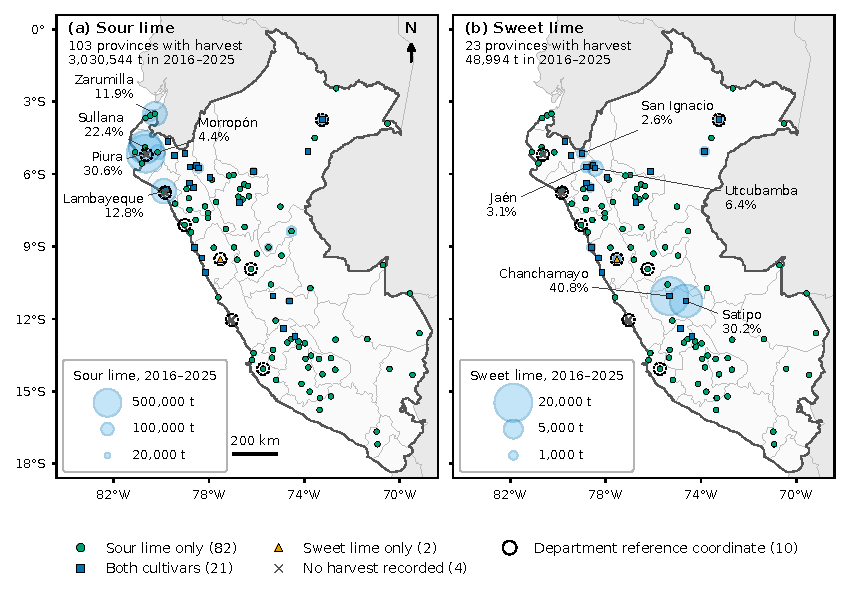
\includegraphics[width=\linewidth,height=0.8\textheight,keepaspectratio]{fig29_study_area_map.pdf}
\caption{\figcap{fig29_study_area_map}}
\label{fig:fig29_study_area_map}
\end{figure}

\begin{figure}[htbp]
\centering
\begin{subfigure}{\linewidth}
\centering
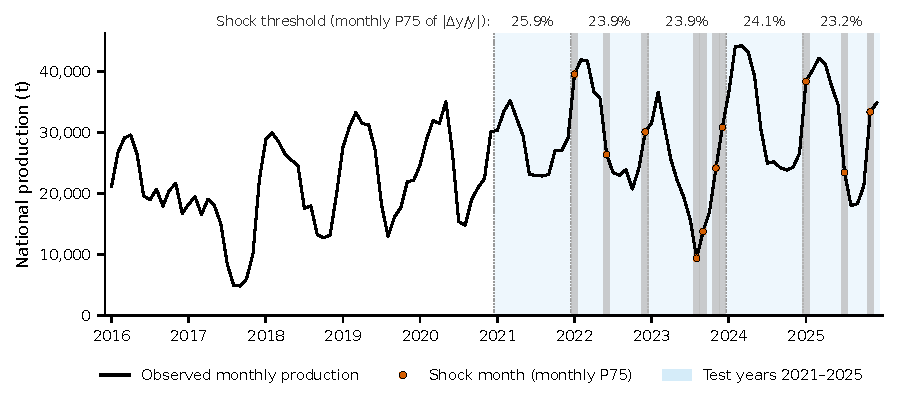
\includegraphics[width=\linewidth,height=0.36\textheight,keepaspectratio]{fig24_series_with_shocks_sutil.pdf}
\caption{Sour lime}
\label{fig:fig24_series_with_shocks_sutil}
\end{subfigure}
\par\medskip
\begin{subfigure}{\linewidth}
\centering
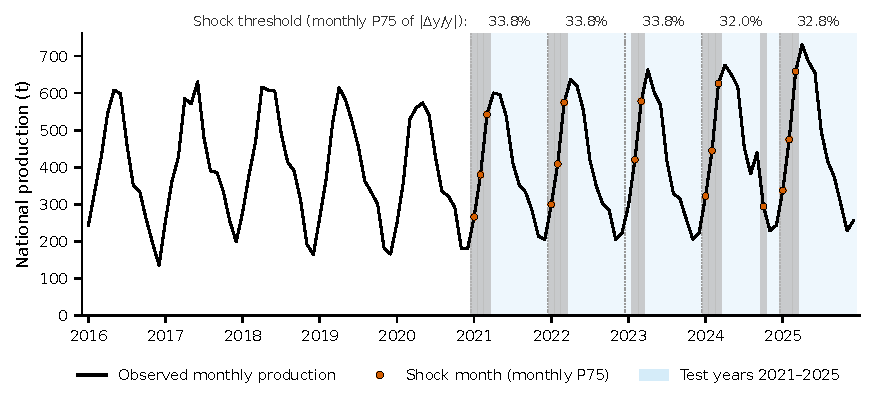
\includegraphics[width=\linewidth,height=0.36\textheight,keepaspectratio]{fig24_series_with_shocks_dulce.pdf}
\caption{Sweet lime}
\label{fig:fig24_series_with_shocks_dulce}
\end{subfigure}
\caption{\textit{Sour lime:} \figcap{fig24_series_with_shocks_sutil} \textit{Sweet lime:} \figcap{fig24_series_with_shocks_dulce}}
\label{fig:fig24_series_with_shocks}
\end{figure}

\begin{figure}[htbp]
\centering
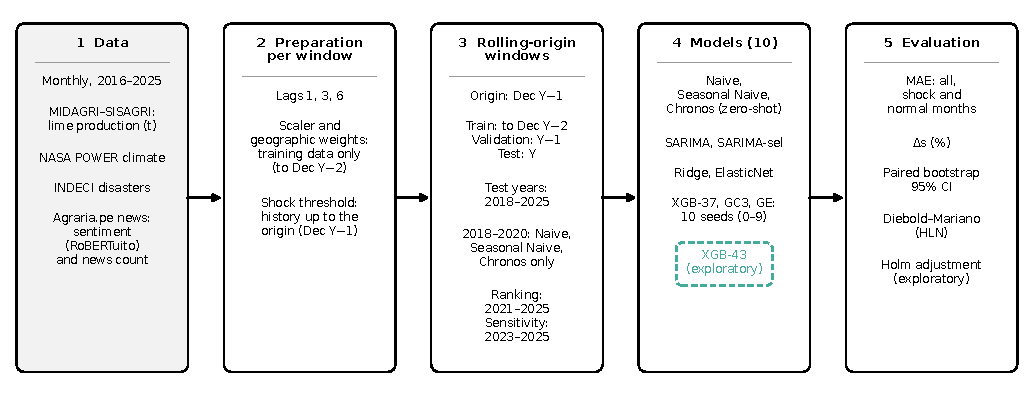
\includegraphics[width=\linewidth,height=0.8\textheight,keepaspectratio]{fig_workflow.pdf}
\caption{\figcap{fig_workflow}}
\label{fig:fig_workflow}
\end{figure}

\begin{figure}[htbp]
\centering
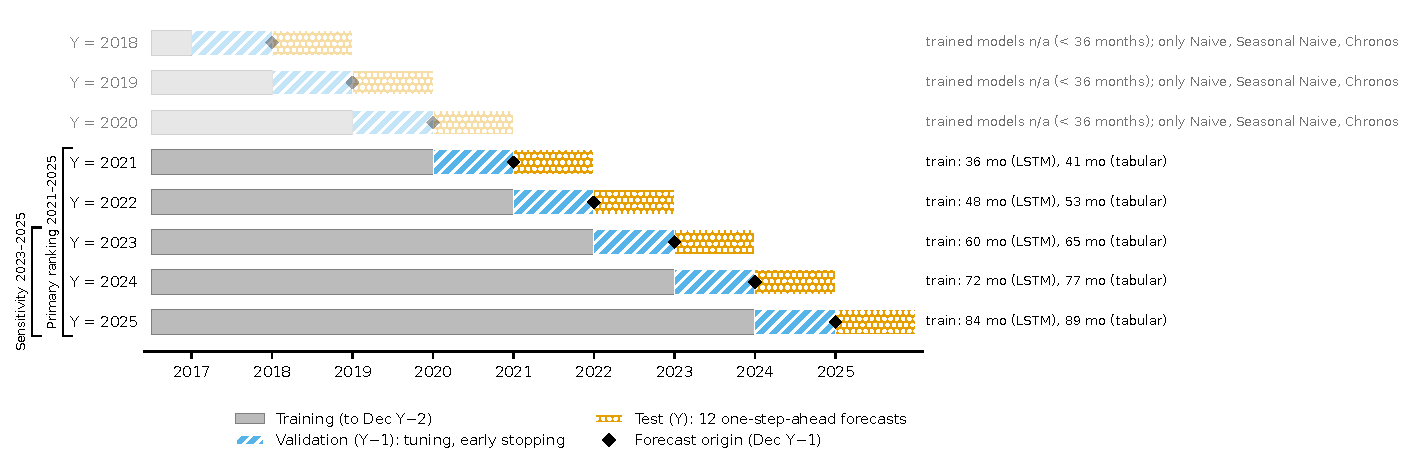
\includegraphics[width=\linewidth,height=0.8\textheight,keepaspectratio]{fig30_rolling_origin_scheme.pdf}
\caption{\figcap{fig30_rolling_origin_scheme}}
\label{fig:fig30_rolling_origin_scheme}
\end{figure}

\begin{figure}[htbp]
\centering
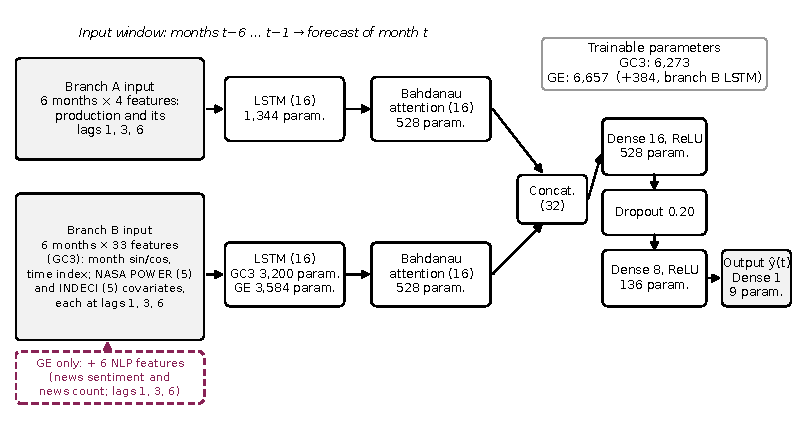
\includegraphics[width=\linewidth,height=0.8\textheight,keepaspectratio]{fig25_architecture_dual_lstm.pdf}
\caption{\figcap{fig25_architecture_dual_lstm}}
\label{fig:fig25_architecture_dual_lstm}
\end{figure}

\begin{figure}[htbp]
\centering
\begin{subfigure}{\linewidth}
\centering
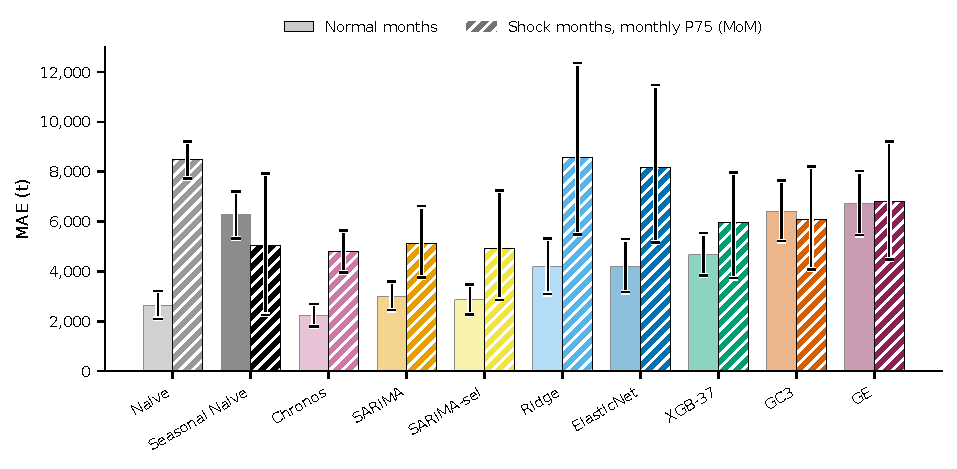
\includegraphics[width=\linewidth,height=0.36\textheight,keepaspectratio]{fig13_mae_normal_vs_shock_bars_sutil.pdf}
\caption{Sour lime}
\label{fig:fig13_mae_normal_vs_shock_bars_sutil}
\end{subfigure}
\par\medskip
\begin{subfigure}{\linewidth}
\centering
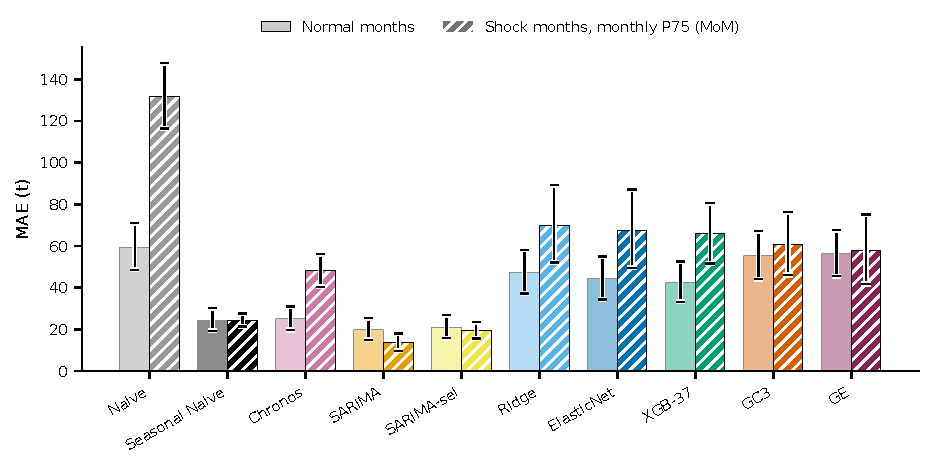
\includegraphics[width=\linewidth,height=0.36\textheight,keepaspectratio]{fig13_mae_normal_vs_shock_bars_dulce.pdf}
\caption{Sweet lime}
\label{fig:fig13_mae_normal_vs_shock_bars_dulce}
\end{subfigure}
\caption{\textit{Sour lime:} \figcap{fig13_mae_normal_vs_shock_bars_sutil} \textit{Sweet lime:} \figcap{fig13_mae_normal_vs_shock_bars_dulce}}
\label{fig:fig13_mae_normal_vs_shock_bars}
\end{figure}

\begin{figure}[htbp]
\centering
\begin{subfigure}{\linewidth}
\centering
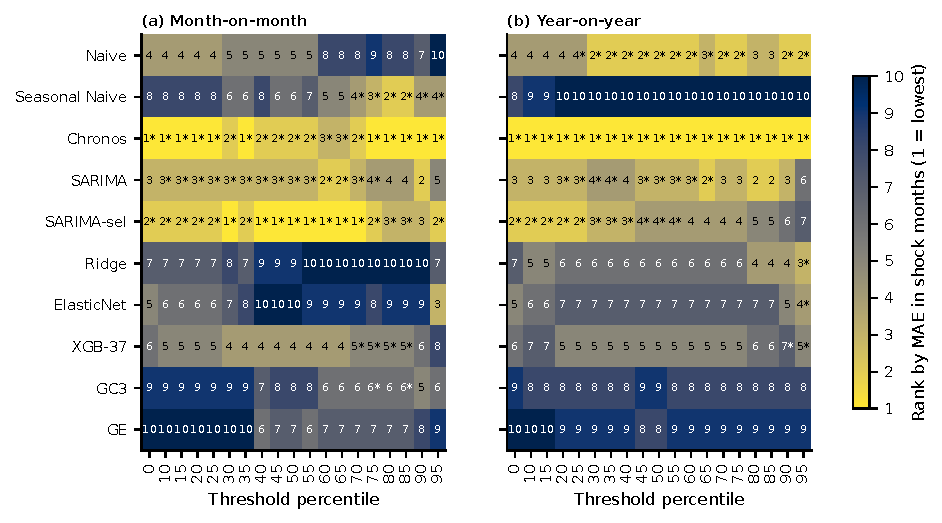
\includegraphics[width=\linewidth,height=0.36\textheight,keepaspectratio]{fig07_rank_heatmap_model_percentile_sutil.pdf}
\caption{Sour lime}
\label{fig:fig07_rank_heatmap_model_percentile_sutil}
\end{subfigure}
\par\medskip
\begin{subfigure}{\linewidth}
\centering
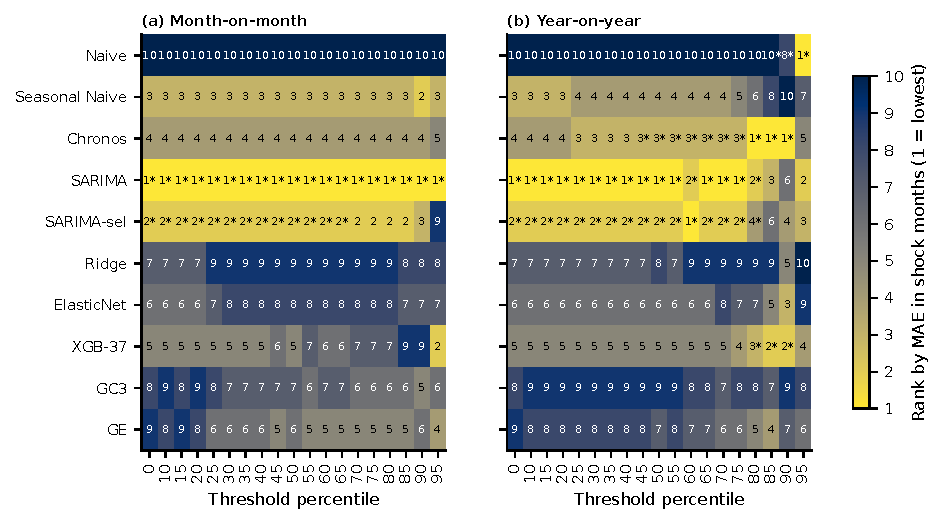
\includegraphics[width=\linewidth,height=0.36\textheight,keepaspectratio]{fig07_rank_heatmap_model_percentile_dulce.pdf}
\caption{Sweet lime}
\label{fig:fig07_rank_heatmap_model_percentile_dulce}
\end{subfigure}
\caption{\textit{Sour lime:} \figcap{fig07_rank_heatmap_model_percentile_sutil} \textit{Sweet lime:} \figcap{fig07_rank_heatmap_model_percentile_dulce}}
\label{fig:fig07_rank_heatmap_model_percentile}
\end{figure}

\begin{figure}[htbp]
\centering
\begin{subfigure}{\linewidth}
\centering
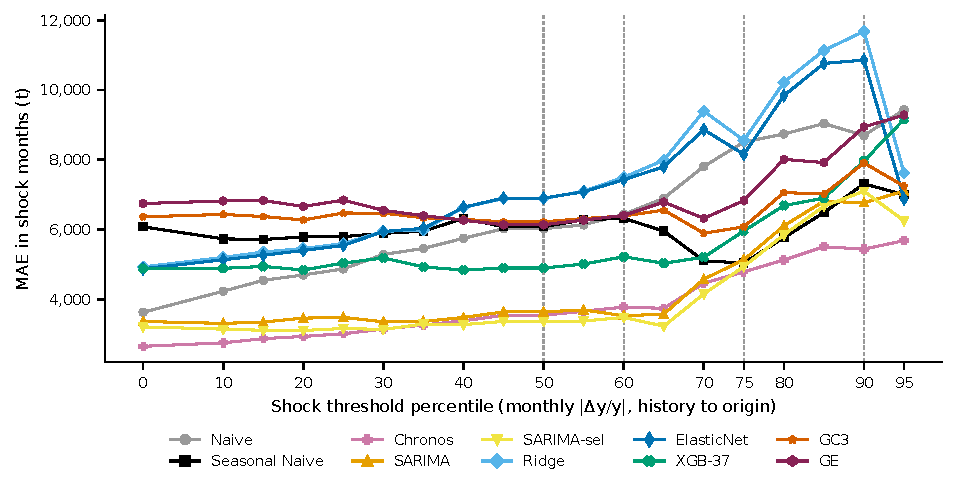
\includegraphics[width=\linewidth,height=0.36\textheight,keepaspectratio]{fig05_mae_shock_vs_percentile_sutil.pdf}
\caption{Sour lime}
\label{fig:fig05_mae_shock_vs_percentile_sutil}
\end{subfigure}
\par\medskip
\begin{subfigure}{\linewidth}
\centering
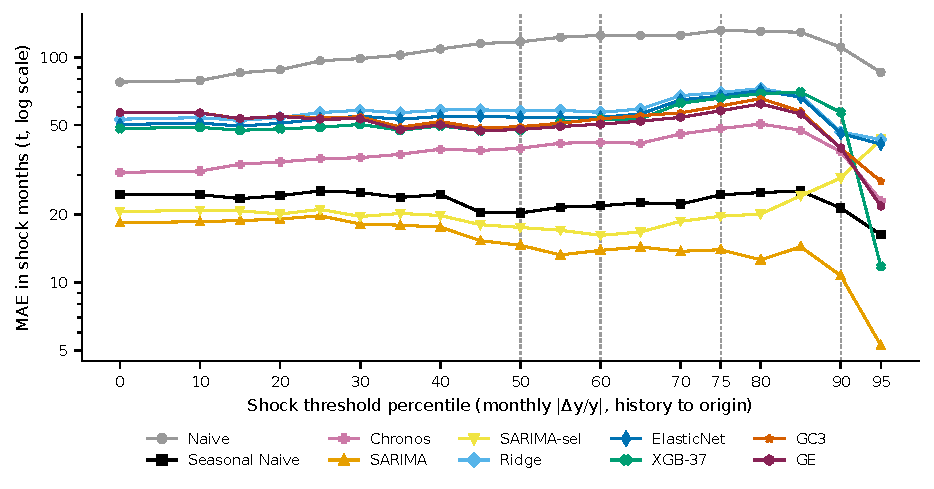
\includegraphics[width=\linewidth,height=0.36\textheight,keepaspectratio]{fig05_mae_shock_vs_percentile_dulce.pdf}
\caption{Sweet lime}
\label{fig:fig05_mae_shock_vs_percentile_dulce}
\end{subfigure}
\caption{\textit{Sour lime:} \figcap{fig05_mae_shock_vs_percentile_sutil} \textit{Sweet lime:} \figcap{fig05_mae_shock_vs_percentile_dulce}}
\label{fig:fig05_mae_shock_vs_percentile}
\end{figure}

\begin{figure}[htbp]
\centering
\begin{subfigure}{\linewidth}
\centering
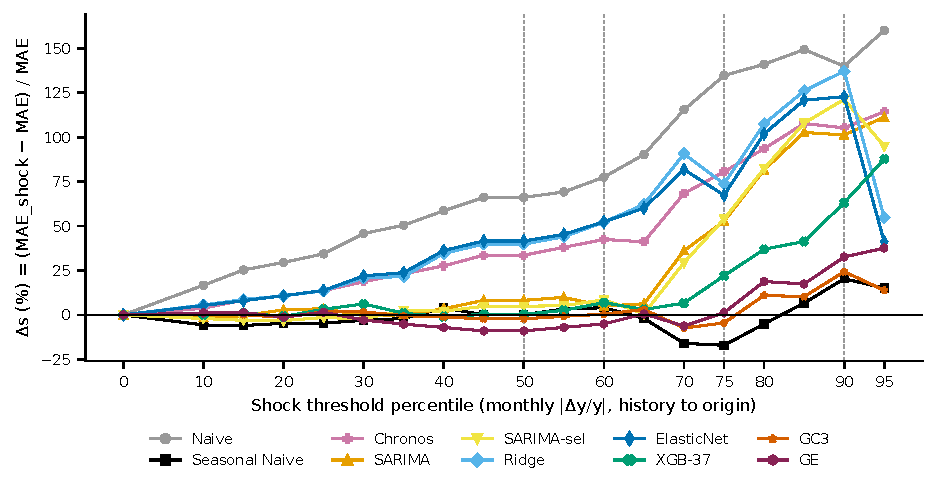
\includegraphics[width=\linewidth,height=0.36\textheight,keepaspectratio]{fig04_delta_s_vs_percentile_sutil.pdf}
\caption{Sour lime}
\label{fig:fig04_delta_s_vs_percentile_sutil}
\end{subfigure}
\par\medskip
\begin{subfigure}{\linewidth}
\centering
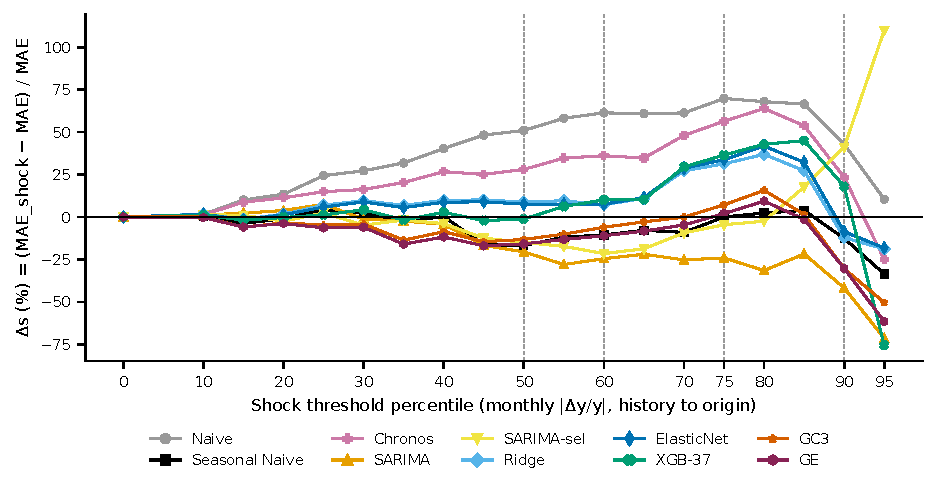
\includegraphics[width=\linewidth,height=0.36\textheight,keepaspectratio]{fig04_delta_s_vs_percentile_dulce.pdf}
\caption{Sweet lime}
\label{fig:fig04_delta_s_vs_percentile_dulce}
\end{subfigure}
\caption{\textit{Sour lime:} \figcap{fig04_delta_s_vs_percentile_sutil} \textit{Sweet lime:} \figcap{fig04_delta_s_vs_percentile_dulce}}
\label{fig:fig04_delta_s_vs_percentile}
\end{figure}

\begin{figure}[htbp]
\centering
\begin{subfigure}{\linewidth}
\centering
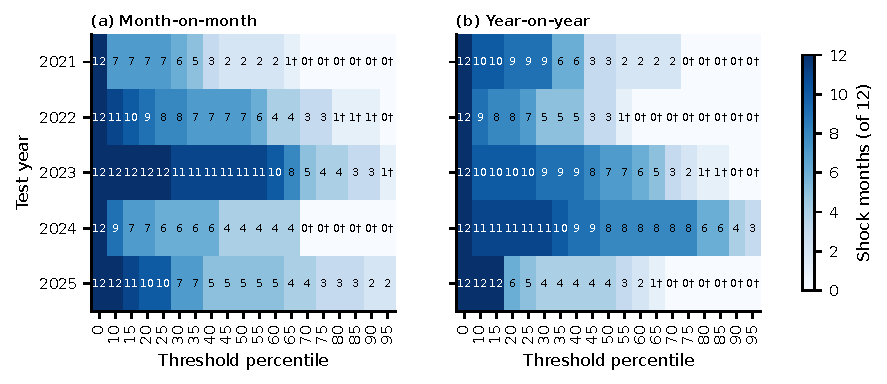
\includegraphics[width=\linewidth,height=0.36\textheight,keepaspectratio]{fig10_n_shock_heatmap_window_percentile_sutil.pdf}
\caption{Sour lime}
\label{fig:fig10_n_shock_heatmap_window_percentile_sutil}
\end{subfigure}
\par\medskip
\begin{subfigure}{\linewidth}
\centering
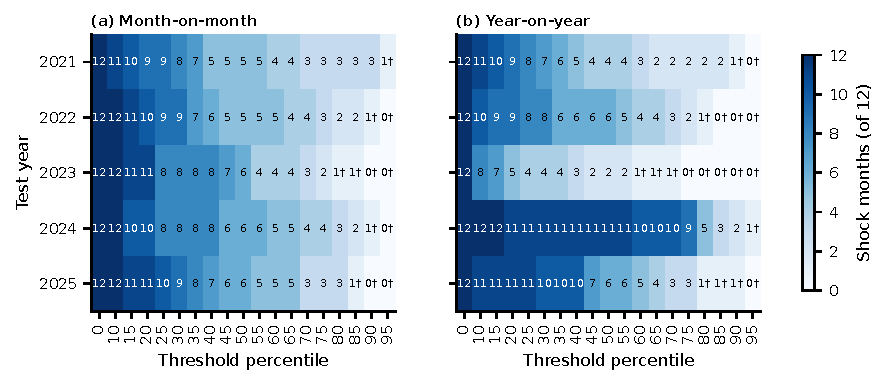
\includegraphics[width=\linewidth,height=0.36\textheight,keepaspectratio]{fig10_n_shock_heatmap_window_percentile_dulce.pdf}
\caption{Sweet lime}
\label{fig:fig10_n_shock_heatmap_window_percentile_dulce}
\end{subfigure}
\caption{\textit{Sour lime:} \figcap{fig10_n_shock_heatmap_window_percentile_sutil} \textit{Sweet lime:} \figcap{fig10_n_shock_heatmap_window_percentile_dulce}}
\label{fig:fig10_n_shock_heatmap_window_percentile}
\end{figure}

\begin{figure}[htbp]
\centering
\begin{subfigure}{\linewidth}
\centering
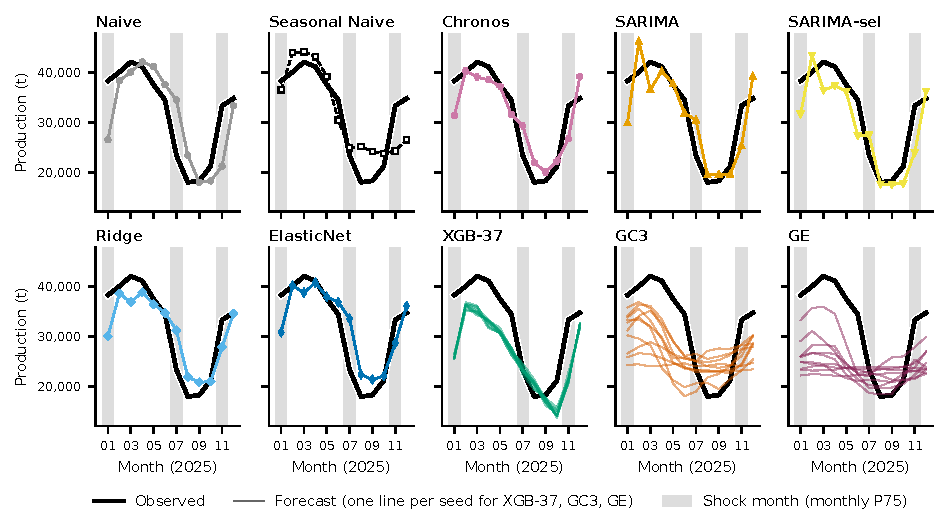
\includegraphics[width=\linewidth,height=0.36\textheight,keepaspectratio]{fig20_real_vs_pred_2025_sutil.pdf}
\caption{Sour lime}
\label{fig:fig20_real_vs_pred_2025_sutil}
\end{subfigure}
\par\medskip
\begin{subfigure}{\linewidth}
\centering
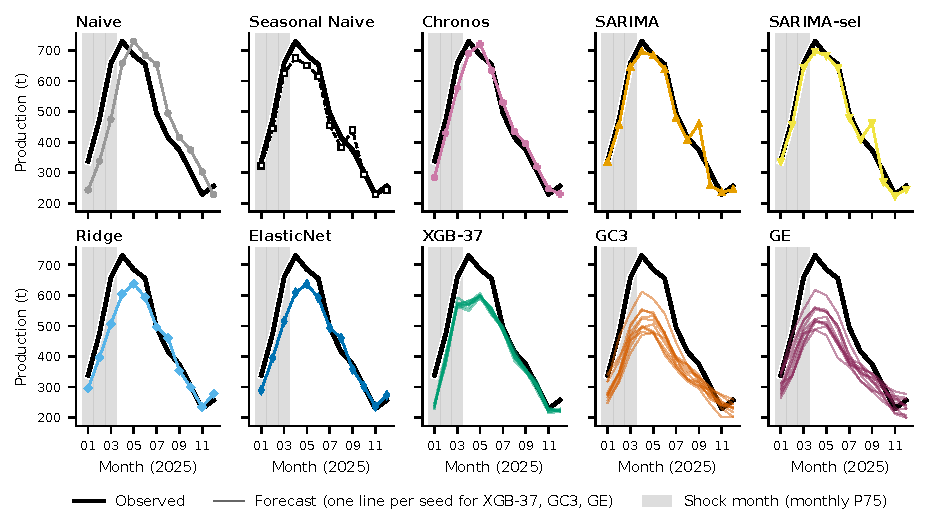
\includegraphics[width=\linewidth,height=0.36\textheight,keepaspectratio]{fig20_real_vs_pred_2025_dulce.pdf}
\caption{Sweet lime}
\label{fig:fig20_real_vs_pred_2025_dulce}
\end{subfigure}
\caption{\textit{Sour lime:} \figcap{fig20_real_vs_pred_2025_sutil} \textit{Sweet lime:} \figcap{fig20_real_vs_pred_2025_dulce}}
\label{fig:fig20_real_vs_pred_2025}
\end{figure}

\begin{figure}[htbp]
\centering
\begin{subfigure}{\linewidth}
\centering
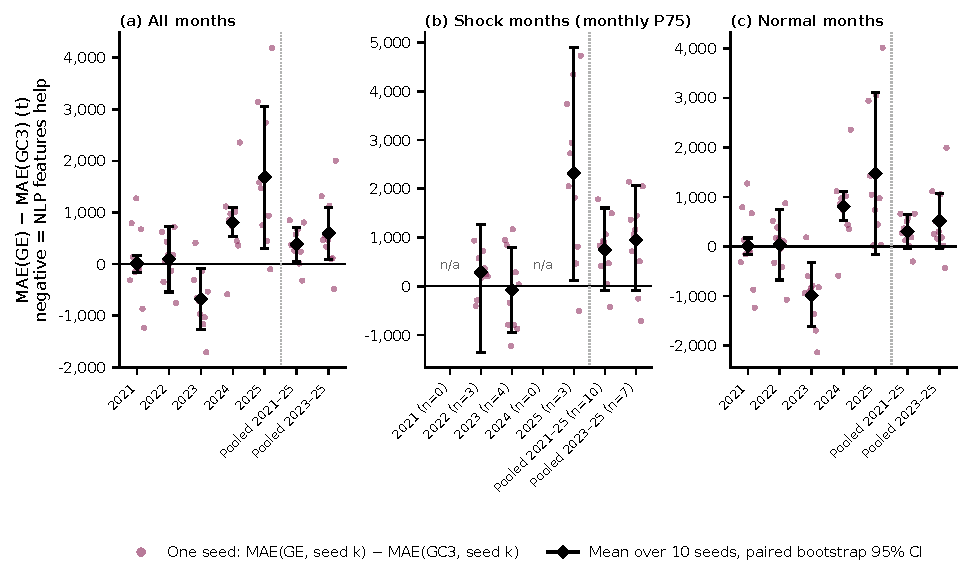
\includegraphics[width=\linewidth,height=0.36\textheight,keepaspectratio]{fig18_nlp_ablation_paired_sutil.pdf}
\caption{Sour lime}
\label{fig:fig18_nlp_ablation_paired_sutil}
\end{subfigure}
\par\medskip
\begin{subfigure}{\linewidth}
\centering
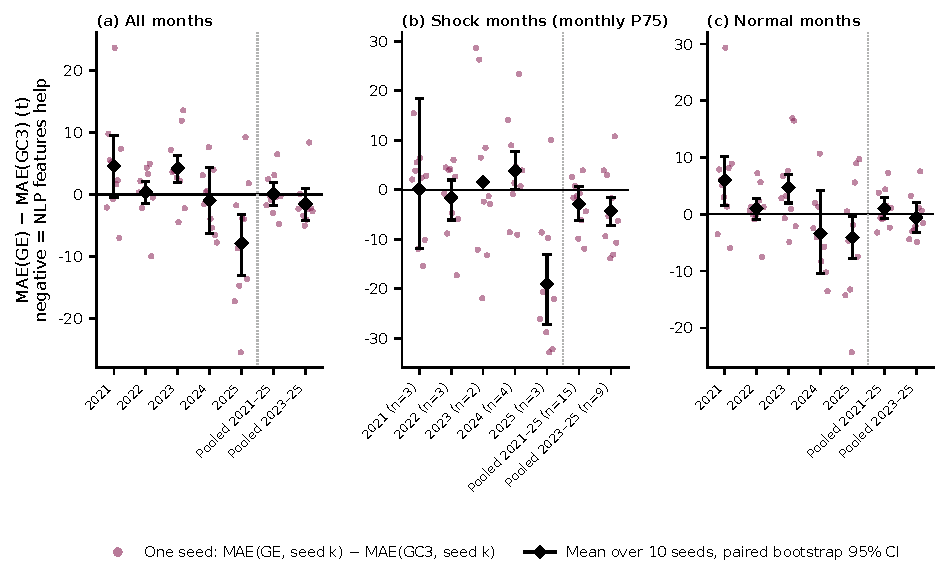
\includegraphics[width=\linewidth,height=0.36\textheight,keepaspectratio]{fig18_nlp_ablation_paired_dulce.pdf}
\caption{Sweet lime}
\label{fig:fig18_nlp_ablation_paired_dulce}
\end{subfigure}
\caption{\textit{Sour lime:} \figcap{fig18_nlp_ablation_paired_sutil} \textit{Sweet lime:} \figcap{fig18_nlp_ablation_paired_dulce}}
\label{fig:fig18_nlp_ablation_paired}
\end{figure}

\begin{figure}[htbp]
\centering
\begin{subfigure}{\linewidth}
\centering
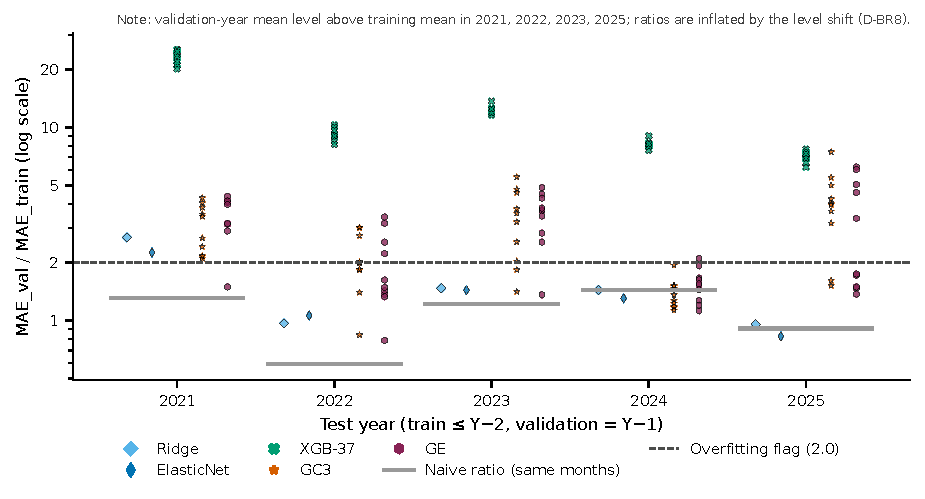
\includegraphics[width=\linewidth,height=0.36\textheight,keepaspectratio]{fig02_train_val_gap_sutil.pdf}
\caption{Sour lime}
\label{fig:fig02_train_val_gap_sutil}
\end{subfigure}
\par\medskip
\begin{subfigure}{\linewidth}
\centering
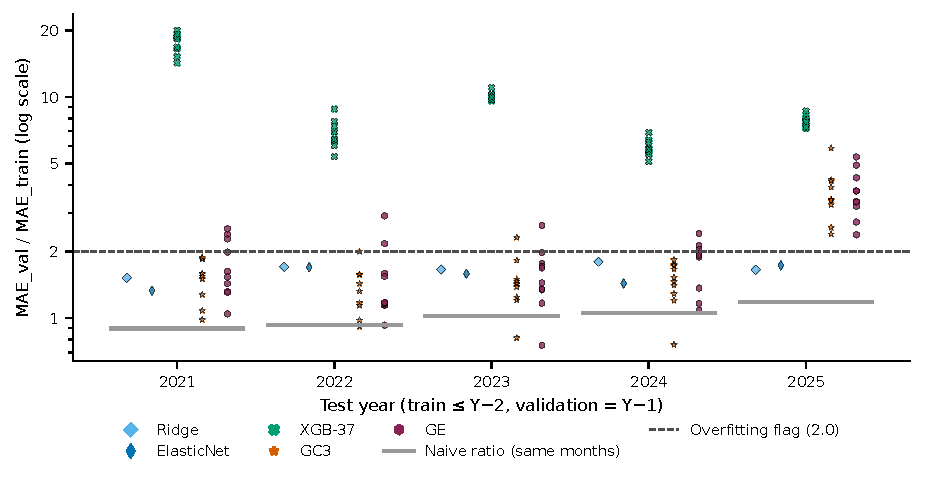
\includegraphics[width=\linewidth,height=0.36\textheight,keepaspectratio]{fig02_train_val_gap_dulce.pdf}
\caption{Sweet lime}
\label{fig:fig02_train_val_gap_dulce}
\end{subfigure}
\caption{\textit{Sour lime:} \figcap{fig02_train_val_gap_sutil} \textit{Sweet lime:} \figcap{fig02_train_val_gap_dulce}}
\label{fig:fig02_train_val_gap}
\end{figure}

% ===== SUPLEMENTARIO =====

% ===== tables_supp.tex =====
% Tables, supplementary material, in order of appearance.

\begin{landscape}
\scriptsize
\setlength{\tabcolsep}{3pt}
% --- tables/TS1_provinces.tex
\begin{longtable}{llrrllrrrrrr}
\caption{Lime-producing provinces of Peru, January 2016–December 2025 (MIDAGRI–SISAGRI (accessed \midagridate{})). Shares are relative to the national total of each cultivar; months with production count the months with production $>$ 0 out of 120.} \label{tab:S1_provinces} \\
\toprule
Department & Province & Latitude & Longitude & Coordinate & Category & Sour lime 2016-2025 (t) & Sour lime share (\%) & Months with sour lime $>$ 0 (of 120) & Sweet lime 2016-2025 (t) & Sweet lime share (\%) & Months with sweet lime $>$ 0 (of 120) \\
\midrule
\endfirsthead
\caption[]{Lime-producing provinces of Peru, January 2016–December 2025 (MIDAGRI–SISAGRI (accessed \midagridate{})). Shares are relative to the national total of each cultivar; months with production count the months with production $>$ 0 out of 120.} \\
\toprule
Department & Province & Latitude & Longitude & Coordinate & Category & Sour lime 2016-2025 (t) & Sour lime share (\%) & Months with sour lime $>$ 0 (of 120) & Sweet lime 2016-2025 (t) & Sweet lime share (\%) & Months with sweet lime $>$ 0 (of 120) \\
\midrule
\endhead
\midrule
\multicolumn{12}{r}{Continued on next page} \\
\midrule
\endfoot
\bottomrule
\endlastfoot
PIURA & PIURA & -5.15 & -80.66 & province & Sour lime only & 926,666.00 & 30.58 & 120.00 & 0.00 & 0.00 & 0.00 \\
PIURA & SULLANA & -4.89 & -80.69 & province & Sour lime only & 678,010.00 & 22.37 & 120.00 & 0.00 & 0.00 & 0.00 \\
LAMBAYEQUE & LAMBAYEQUE & -6.71 & -79.90 & province & Sour lime only & 386,555.00 & 12.76 & 120.00 & 0.00 & 0.00 & 0.00 \\
TUMBES & ZARUMILLA & -3.50 & -80.28 & province & Sour lime only & 361,442.10 & 11.93 & 120.00 & 0.00 & 0.00 & 0.00 \\
PIURA & MORROPON & -5.10 & -80.16 & province & Sour lime only & 132,988.00 & 4.39 & 120.00 & 0.00 & 0.00 & 0.00 \\
TUMBES & TUMBES & -3.57 & -80.46 & province & Sour lime only & 74,185.40 & 2.45 & 120.00 & 0.00 & 0.00 & 0.00 \\
UCAYALI & CORONEL PORTILLO & -8.37 & -74.54 & province & Sour lime only & 61,919.70 & 2.04 & 120.00 & 0.00 & 0.00 & 0.00 \\
LORETO & MAYNAS & -3.75 & -73.24 & province & Both cultivars & 55,277.00 & 1.82 & 120.00 & 942.00 & 1.92 & 40.00 \\
AMAZONAS & UTCUBAMBA & -5.75 & -78.44 & province & Both cultivars & 52,073.80 & 1.72 & 120.00 & 3,150.10 & 6.43 & 120.00 \\
UCAYALI & PADRE ABAD & -9.03 & -75.51 & province & Sour lime only & 32,399.90 & 1.07 & 120.00 & 0.00 & 0.00 & 0.00 \\
LORETO & ALTO AMAZONAS & -5.88 & -76.13 & province & Both cultivars & 26,941.00 & 0.89 & 120.00 & 67.00 & 0.14 & 39.00 \\
JUNIN & SATIPO & -11.25 & -74.64 & province & Both cultivars & 25,734.80 & 0.85 & 120.00 & 14,818.60 & 30.25 & 104.00 \\
TUMBES & CONTRALMIRANTE VILLAR & -3.68 & -80.67 & province & Sour lime only & 16,441.30 & 0.54 & 120.00 & 0.00 & 0.00 & 0.00 \\
CUSCO & LA CONVENCION & -12.86 & -72.69 & province & Sour lime only & 16,102.80 & 0.53 & 118.00 & 0.00 & 0.00 & 0.00 \\
UCAYALI & ATALAYA & -10.73 & -73.76 & province & Sour lime only & 16,010.20 & 0.53 & 120.00 & 0.00 & 0.00 & 0.00 \\
LORETO & UCAYALI & -7.35 & -75.01 & province & Sour lime only & 10,926.00 & 0.36 & 120.00 & 0.00 & 0.00 & 0.00 \\
SAN MARTIN & SAN MARTIN & -6.49 & -76.36 & province & Sour lime only & 9,544.10 & 0.31 & 120.00 & 0.00 & 0.00 & 0.00 \\
SAN MARTIN & PICOTA & -6.92 & -76.33 & province & Sour lime only & 8,634.60 & 0.28 & 120.00 & 0.00 & 0.00 & 0.00 \\
HUANUCO & LEONCIO PRADO & -9.30 & -76.00 & province & Sour lime only & 8,021.60 & 0.26 & 119.00 & 0.00 & 0.00 & 0.00 \\
SAN MARTIN & LAMAS & -6.42 & -76.52 & province & Sour lime only & 7,705.30 & 0.25 & 120.00 & 0.00 & 0.00 & 0.00 \\
JUNIN & CHANCHAMAYO & -11.06 & -75.33 & province & Both cultivars & 7,518.10 & 0.25 & 120.00 & 20,007.60 & 40.84 & 120.00 \\
ICA & ICA & -14.06 & -75.73 & province & Sour lime only & 6,788.40 & 0.22 & 74.00 & 0.00 & 0.00 & 0.00 \\
LORETO & LORETO & -4.50 & -73.57 & province & Sour lime only & 5,785.00 & 0.19 & 120.00 & 0.00 & 0.00 & 0.00 \\
SAN MARTIN & HUALLAGA & -6.94 & -76.77 & province & Sour lime only & 4,744.00 & 0.16 & 120.00 & 0.00 & 0.00 & 0.00 \\
LORETO & MARISCAL RAMON CASTILLA & -3.91 & -70.52 & province & Sour lime only & 4,463.00 & 0.15 & 110.00 & 0.00 & 0.00 & 0.00 \\
ANCASH & CASMA & -9.48 & -78.31 & province & Both cultivars & 4,240.00 & 0.14 & 120.00 & 358.00 & 0.73 & 74.00 \\
LORETO & REQUENA & -5.06 & -73.86 & province & Both cultivars & 3,935.00 & 0.13 & 120.00 & 1,094.00 & 2.23 & 120.00 \\
ICA & PISCO & -13.71 & -76.20 & province & Sour lime only & 3,862.80 & 0.13 & 54.00 & 0.00 & 0.00 & 0.00 \\
ICA & NASCA & -14.07 & -75.73 & department reference & Sour lime only & 3,794.00 & 0.13 & 31.00 & 0.00 & 0.00 & 0.00 \\
MADRE DE DIOS & TAMBOPATA & -12.59 & -69.18 & province & Sour lime only & 3,780.20 & 0.12 & 120.00 & 0.00 & 0.00 & 0.00 \\
SAN MARTIN & MARISCAL CACERES & -7.18 & -76.72 & province & Both cultivars & 3,678.70 & 0.12 & 111.00 & 199.80 & 0.41 & 84.00 \\
PIURA & AYABACA & -4.64 & -79.72 & province & Both cultivars & 3,610.90 & 0.12 & 113.00 & 1.00 & 0.00 & 1.00 \\
LORETO & DATEM DEL MARAÑON & -3.75 & -73.25 & department reference & Sour lime only & 3,254.00 & 0.11 & 110.00 & 0.00 & 0.00 & 0.00 \\
SAN MARTIN & BELLAVISTA & -7.05 & -76.59 & province & Sour lime only & 3,180.00 & 0.10 & 120.00 & 0.00 & 0.00 & 0.00 \\
SAN MARTIN & MOYOBAMBA & -6.03 & -76.97 & province & Sour lime only & 2,903.80 & 0.10 & 84.00 & 0.00 & 0.00 & 0.00 \\
SAN MARTIN & TOCACHE & -8.19 & -76.51 & province & Sour lime only & 2,898.80 & 0.10 & 109.00 & 0.00 & 0.00 & 0.00 \\
AMAZONAS & LUYA & -6.14 & -77.95 & province & Both cultivars & 2,812.70 & 0.09 & 120.00 & 330.90 & 0.68 & 120.00 \\
AMAZONAS & BAGUA & -5.64 & -78.53 & province & Both cultivars & 2,484.90 & 0.08 & 120.00 & 951.70 & 1.94 & 120.00 \\
AMAZONAS & CHACHAPOYAS & -6.23 & -77.87 & province & Sour lime only & 2,427.00 & 0.08 & 120.00 & 0.00 & 0.00 & 0.00 \\
SAN MARTIN & RIOJA & -6.06 & -77.17 & province & Sour lime only & 2,318.80 & 0.08 & 109.00 & 0.00 & 0.00 & 0.00 \\
PIURA & HUANCABAMBA & -5.24 & -79.45 & province & Both cultivars & 2,031.20 & 0.07 & 118.00 & 30.20 & 0.06 & 9.00 \\
UCAYALI & PURUS & -9.77 & -70.71 & province & Sour lime only & 2,029.80 & 0.07 & 120.00 & 0.00 & 0.00 & 0.00 \\
CAJAMARCA & SAN MIGUEL & -7.00 & -78.85 & province & Sour lime only & 1,909.70 & 0.06 & 77.00 & 0.00 & 0.00 & 0.00 \\
SAN MARTIN & EL DORADO & -6.61 & -76.70 & province & Sour lime only & 1,855.70 & 0.06 & 114.00 & 0.00 & 0.00 & 0.00 \\
LA LIBERTAD & VIRU & -8.41 & -78.75 & province & Sour lime only & 1,720.90 & 0.06 & 120.00 & 0.00 & 0.00 & 0.00 \\
ANCASH & HUAYLAS & -9.05 & -77.80 & province & Sour lime only & 1,701.00 & 0.06 & 120.00 & 0.00 & 0.00 & 0.00 \\
CAJAMARCA & CHOTA & -6.56 & -78.65 & province & Both cultivars & 1,634.00 & 0.05 & 92.00 & 956.00 & 1.95 & 77.00 \\
HUANUCO & HUAMALIES & -9.55 & -76.82 & province & Sour lime only & 1,543.50 & 0.05 & 118.00 & 0.00 & 0.00 & 0.00 \\
PIURA & PAITA & -5.09 & -81.10 & province & Sour lime only & 1,444.00 & 0.05 & 110.00 & 0.00 & 0.00 & 0.00 \\
MADRE DE DIOS & MANU & -12.84 & -71.37 & province & Sour lime only & 1,404.00 & 0.05 & 120.00 & 0.00 & 0.00 & 0.00 \\
LORETO & PUTUMAYO & -2.45 & -72.67 & province & Sour lime only & 1,398.00 & 0.05 & 120.00 & 0.00 & 0.00 & 0.00 \\
LAMBAYEQUE & FERREÑAFE & -6.64 & -79.79 & province & Both cultivars & 1,376.80 & 0.05 & 54.00 & 71.00 & 0.14 & 10.00 \\
APURIMAC & ABANCAY & -13.63 & -72.89 & province & Sour lime only & 1,375.00 & 0.05 & 113.00 & 0.00 & 0.00 & 0.00 \\
CAJAMARCA & JAEN & -5.71 & -78.81 & province & Both cultivars & 1,253.30 & 0.04 & 120.00 & 1,528.10 & 3.12 & 96.00 \\
MADRE DE DIOS & TAHUAMANU & -10.95 & -69.58 & province & Sour lime only & 1,240.40 & 0.04 & 120.00 & 0.00 & 0.00 & 0.00 \\
JUNIN & HUANCAYO & -12.07 & -75.21 & province & Sour lime only & 1,196.70 & 0.04 & 120.00 & 0.00 & 0.00 & 0.00 \\
AYACUCHO & LA MAR & -13.01 & -73.98 & province & Sour lime only & 1,176.80 & 0.04 & 113.00 & 0.00 & 0.00 & 0.00 \\
PASCO & OXAPAMPA & -10.57 & -75.40 & province & Sour lime only & 1,030.30 & 0.03 & 28.00 & 0.00 & 0.00 & 0.00 \\
HUANCAVELICA & TAYACAJA & -12.40 & -74.87 & province & Both cultivars & 952.10 & 0.03 & 52.00 & 170.70 & 0.35 & 27.00 \\
LA LIBERTAD & BOLIVAR & -7.15 & -77.70 & province & Sour lime only & 799.80 & 0.03 & 104.00 & 0.00 & 0.00 & 0.00 \\
APURIMAC & CHINCHEROS & -13.52 & -73.72 & province & Sour lime only & 787.40 & 0.03 & 43.00 & 0.00 & 0.00 & 0.00 \\
APURIMAC & ANDAHUAYLAS & -13.66 & -73.39 & province & Sour lime only & 751.40 & 0.02 & 46.00 & 0.00 & 0.00 & 0.00 \\
HUANUCO & HUANUCO & -9.93 & -76.24 & province & Sour lime only & 676.60 & 0.02 & 115.00 & 0.00 & 0.00 & 0.00 \\
LA LIBERTAD & PATAZ & -8.28 & -77.30 & province & Sour lime only & 664.10 & 0.02 & 91.00 & 0.00 & 0.00 & 0.00 \\
CAJAMARCA & CAJABAMBA & -7.62 & -78.05 & province & Sour lime only & 661.90 & 0.02 & 118.00 & 0.00 & 0.00 & 0.00 \\
AYACUCHO & HUANTA & -12.94 & -74.25 & province & Sour lime only & 656.50 & 0.02 & 83.00 & 0.00 & 0.00 & 0.00 \\
ANCASH & SANTA & -9.04 & -78.61 & province & Both cultivars & 634.00 & 0.02 & 119.00 & 910.00 & 1.86 & 112.00 \\
ANCASH & HUARMEY & -10.07 & -78.15 & province & Both cultivars & 537.00 & 0.02 & 115.00 & 301.00 & 0.61 & 72.00 \\
AYACUCHO & LUCANAS & -14.69 & -74.12 & province & Sour lime only & 534.00 & 0.02 & 54.00 & 0.00 & 0.00 & 0.00 \\
HUANUCO & PUERTO INCA & -9.38 & -74.97 & province & Sour lime only & 520.60 & 0.02 & 110.00 & 0.00 & 0.00 & 0.00 \\
HUANUCO & HUACAYBAMBA & -9.04 & -76.95 & province & Sour lime only & 507.20 & 0.02 & 46.00 & 0.00 & 0.00 & 0.00 \\
LA LIBERTAD & CHEPEN & -7.23 & -79.43 & province & Sour lime only & 499.50 & 0.02 & 67.00 & 0.00 & 0.00 & 0.00 \\
AYACUCHO & PAUCAR DEL SARA SARA & -15.28 & -73.34 & province & Sour lime only & 496.00 & 0.02 & 44.00 & 0.00 & 0.00 & 0.00 \\
AYACUCHO & VILCAS HUAMAN & -13.65 & -73.95 & province & Sour lime only & 479.60 & 0.02 & 69.00 & 0.00 & 0.00 & 0.00 \\
LA LIBERTAD & SANCHEZ CARRION & -7.81 & -78.05 & province & Sour lime only & 465.80 & 0.02 & 108.00 & 0.00 & 0.00 & 0.00 \\
PIURA & SECHURA & -5.56 & -80.82 & province & Sour lime only & 464.00 & 0.02 & 109.00 & 0.00 & 0.00 & 0.00 \\
PUNO & SANDIA & -14.32 & -69.47 & province & Sour lime only & 459.70 & 0.02 & 51.00 & 0.00 & 0.00 & 0.00 \\
HUANUCO & MARAÑON & -9.93 & -76.24 & department reference & Sour lime only & 458.50 & 0.02 & 80.00 & 0.00 & 0.00 & 0.00 \\
CAJAMARCA & SAN IGNACIO & -5.15 & -79.00 & province & Both cultivars & 425.70 & 0.01 & 76.00 & 1,274.50 & 2.60 & 84.00 \\
MOQUEGUA & GENERAL SANCHEZ CERRO & -16.67 & -70.97 & province & Sour lime only & 394.40 & 0.01 & 37.00 & 0.00 & 0.00 & 0.00 \\
MOQUEGUA & MARISCAL NIETO & -17.19 & -70.93 & province & Sour lime only & 359.70 & 0.01 & 35.00 & 0.00 & 0.00 & 0.00 \\
HUANCAVELICA & CHURCAMPA & -12.74 & -74.39 & province & Both cultivars & 336.40 & 0.01 & 60.00 & 141.90 & 0.29 & 49.00 \\
CAJAMARCA & SAN MARCOS & -7.34 & -78.17 & province & Sour lime only & 324.90 & 0.01 & 108.00 & 0.00 & 0.00 & 0.00 \\
LIMA & HUAURA & -11.11 & -77.61 & province & Sour lime only & 308.90 & 0.01 & 20.00 & 0.00 & 0.00 & 0.00 \\
CAJAMARCA & SANTA CRUZ & -6.63 & -78.94 & province & Sour lime only & 305.00 & 0.01 & 50.00 & 0.00 & 0.00 & 0.00 \\
AREQUIPA & LA UNION & -15.21 & -72.89 & province & Sour lime only & 281.30 & 0.01 & 10.00 & 0.00 & 0.00 & 0.00 \\
ICA & PALPA & -14.53 & -75.19 & province & Sour lime only & 258.90 & 0.01 & 25.00 & 0.00 & 0.00 & 0.00 \\
HUANCAVELICA & ACOBAMBA & -12.84 & -74.57 & province & Sour lime only & 229.60 & 0.01 & 51.00 & 0.00 & 0.00 & 0.00 \\
APURIMAC & AYMARAES & -14.29 & -73.24 & province & Sour lime only & 189.50 & 0.01 & 117.00 & 0.00 & 0.00 & 0.00 \\
AYACUCHO & SUCRE & -14.01 & -73.84 & province & Sour lime only & 177.00 & 0.01 & 22.00 & 0.00 & 0.00 & 0.00 \\
AYACUCHO & HUAMANGA & -13.16 & -74.23 & province & Sour lime only & 175.20 & 0.01 & 118.00 & 0.00 & 0.00 & 0.00 \\
AREQUIPA & CARAVELI & -15.77 & -73.37 & province & Sour lime only & 165.90 & 0.01 & 17.00 & 0.00 & 0.00 & 0.00 \\
HUANCAVELICA & ANGARAES & -12.98 & -74.72 & province & Sour lime only & 158.90 & 0.01 & 50.00 & 0.00 & 0.00 & 0.00 \\
HUANCAVELICA & HUAYTARA & -13.60 & -75.35 & province & Sour lime only & 150.90 & 0.00 & 66.00 & 0.00 & 0.00 & 0.00 \\
LA LIBERTAD & GRAN CHIMU & -7.48 & -78.82 & province & Sour lime only & 143.90 & 0.00 & 70.00 & 0.00 & 0.00 & 0.00 \\
AYACUCHO & PARINACOCHAS & -15.02 & -73.78 & province & Sour lime only & 131.00 & 0.00 & 40.00 & 0.00 & 0.00 & 0.00 \\
HUANCAVELICA & CASTROVIRREYNA & -13.28 & -75.32 & province & Sour lime only & 127.70 & 0.00 & 79.00 & 0.00 & 0.00 & 0.00 \\
LA LIBERTAD & ASCOPE & -8.11 & -79.03 & department reference & Sour lime only & 121.70 & 0.00 & 52.00 & 0.00 & 0.00 & 0.00 \\
PUNO & CARABAYA & -14.07 & -70.43 & province & Sour lime only & 107.00 & 0.00 & 40.00 & 0.00 & 0.00 & 0.00 \\
LA LIBERTAD & OTUZCO & -7.90 & -78.57 & province & Sour lime only & 106.90 & 0.00 & 73.00 & 0.00 & 0.00 & 0.00 \\
APURIMAC & GRAU & -14.11 & -72.71 & province & Sour lime only & 80.00 & 0.00 & 51.00 & 0.00 & 0.00 & 0.00 \\
ICA & CHINCHA & -13.42 & -76.13 & province & Sour lime only & 76.40 & 0.00 & 13.00 & 0.00 & 0.00 & 0.00 \\
CAJAMARCA & CUTERVO & -6.38 & -78.82 & province & Both cultivars & 21.00 & 0.00 & 4.00 & 309.00 & 0.63 & 37.00 \\
ANCASH & CARHUAZ & -9.53 & -77.53 & department reference & Sweet lime only & 0.00 & 0.00 & 0.00 & 753.00 & 1.54 & 117.00 \\
ANCASH & YUNGAY & -9.53 & -77.53 & department reference & Sweet lime only & 0.00 & 0.00 & 0.00 & 628.00 & 1.28 & 119.00 \\
LAMBAYEQUE & CHICLAYO & -6.77 & -79.84 & department reference & No harvest recorded & 0.00 & 0.00 & 0.00 & 0.00 & 0.00 & 0.00 \\
LIMA & CAÑETE & -12.05 & -77.04 & department reference & No harvest recorded & 0.00 & 0.00 & 0.00 & 0.00 & 0.00 & 0.00 \\
LIMA & LIMA & -12.05 & -77.04 & department reference & No harvest recorded & 0.00 & 0.00 & 0.00 & 0.00 & 0.00 & 0.00 \\
PIURA & TALARA & -5.19 & -80.63 & department reference & No harvest recorded & 0.00 & 0.00 & 0.00 & 0.00 & 0.00 & 0.00 \\
TOTAL &  &  &  &  &  & 3,030,543.60 & 100.00 &  & 48,994.10 & 100.00 &  \\
\end{longtable}
\end{landscape}

% --- tables/T16_exploratorio_xgb43.tex
\begin{table}[H]
\centering
\small
\caption{EXPLORATORY (post-hoc): XGB-43 versus XGB-37, 2021-2025, monthly P75 (t)}
\label{tab:T16_exploratorio_xgb43}
\begin{tabular}{llllllll}
\toprule
Cultivar & Scope & Months & MAE XGB-37 & MAE XGB-43 & XGB-43 $-$ XGB-37 & 95\% CI lower & 95\% CI upper \\
\midrule
sutil & global & 60 & 4,881.4 & 5,011.9 & 130.5 & 1.5 & 260.4 \\
sutil & shock\_P75 & 10 & 5,955.2 & 5,997.2 & 42.0 & -240.1 & 338.3 \\
sutil & normal\_P75 & 50 & 4,666.7 & 4,814.9 & 148.2 & 6.5 & 286.3 \\
dulce & global & 60 & 48.3 & 47.6 & -0.6 & -2.4 & 1.2 \\
dulce & shock\_P75 & 15 & 65.8 & 62.2 & -3.6 & -5.9 & -1.2 \\
dulce & normal\_P75 & 45 & 42.4 & 42.8 & 0.4 & -1.7 & 2.5 \\
\bottomrule
\end{tabular}
\end{table}

% --- tables/T05_MAE_P75_por_ventana_sutil.tex
\begin{table}[H]
\centering
\small
\caption{MAE por ventana, P75 mensual, Sutil (t)}
\label{tab:T05_MAE_P75_por_ventana_sutil}
\begin{tabular}{llllll}
\toprule
modelo & 2021 & 2022 & 2023 & 2024 & 2025 \\
\midrule
Naive & 1,986 & 3,762 & 4,590 & 3,078 & 4,704 \\
Seasonal Naive & 4,590 & 4,136 & 7,638 & 9,850 & 4,160 \\
Chronos & 2,541 & 2,205 & 3,157 & 2,023 & 3,316 \\
SARIMA & 3,208 & 3,061 & 3,693 & 2,858 & 3,985 \\
SARIMA-sel & 2,304 & 2,609 & 3,836 & 3,333 & 3,947 \\
Ridge & 3,108 & 3,187 & 10,778 & 4,322 & 3,232 \\
ElasticNet & 3,006 & 2,968 & 10,413 & 4,751 & 3,223 \\
XGB-37 & 5,211 & 4,552 & 3,785 & 4,957 & 5,902 \\
GC3 & 3,856 & 5,162 & 6,074 & 8,969 & 7,746 \\
GE & 3,867 & 5,260 & 5,391 & 9,774 & 9,426 \\
XGB-43 & 5,333 & 4,664 & 3,679 & 5,466 & 5,918 \\
\bottomrule
\end{tabular}
\end{table}

% --- tables/T05_MAE_P75_por_ventana_dulce.tex
\begin{table}[H]
\centering
\small
\caption{MAE por ventana, P75 mensual, Dulce (t)}
\label{tab:T05_MAE_P75_por_ventana_dulce}
\begin{tabular}{llllll}
\toprule
modelo & 2021 & 2022 & 2023 & 2024 & 2025 \\
\midrule
Naive & 67.8 & 73.3 & 76.2 & 85.6 & 84.7 \\
Seasonal Naive & 18.4 & 19.9 & 11.8 & 41.8 & 30.5 \\
Chronos & 19.2 & 30.0 & 30.4 & 39.9 & 34.6 \\
SARIMA & 13.7 & 12.4 & 18.8 & 25.5 & 21.8 \\
SARIMA-sel & 27.9 & 12.4 & 17.4 & 25.6 & 19.8 \\
Ridge & 37.9 & 35.5 & 43.6 & 97.7 & 50.6 \\
ElasticNet & 37.6 & 35.2 & 43.4 & 85.7 & 49.3 \\
XGB-37 & 25.7 & 52.3 & 45.8 & 58.0 & 59.4 \\
GC3 & 36.5 & 37.2 & 38.0 & 68.2 & 103.4 \\
GE & 41.1 & 37.5 & 42.2 & 67.3 & 95.6 \\
XGB-43 & 26.2 & 52.2 & 44.3 & 54.1 & 61.4 \\
\bottomrule
\end{tabular}
\end{table}

% --- tables/T05_MAE_shock_P75_por_ventana_sutil.tex
\begin{table}[H]
\centering
\small
\caption{MAE\_shock por ventana, P75 mensual, Sutil (t)}
\label{tab:T05_MAE_shock_P75_por_ventana_sutil}
\begin{tabular}{llllll}
\toprule
modelo & 2021 (n=0) & 2022 (n=3) & 2023 (n=4) & 2024 (n=0) & 2025 (n=3) \\
\midrule
Naive & -- & 8,522 & 6,129 & -- & 11,660 \\
Seasonal Naive & -- & 4,472 & 6,135 & -- & 4,130 \\
Chronos & -- & 4,852 & 3,454 & -- & 6,487 \\
SARIMA & -- & 3,905 & 4,030 & -- & 7,824 \\
SARIMA-sel & -- & 4,207 & 4,158 & -- & 6,701 \\
Ridge & -- & 4,394 & 12,714 & -- & 7,177 \\
ElasticNet & -- & 4,015 & 11,806 & -- & 7,423 \\
XGB-37 & -- & 5,234 & 4,740 & -- & 8,297 \\
GC3 & -- & 4,916 & 7,304 & -- & 5,594 \\
GE & -- & 5,202 & 7,234 & -- & 7,908 \\
XGB-43 & -- & 5,374 & 4,656 & -- & 8,408 \\
\bottomrule
\end{tabular}
\end{table}

% --- tables/T05_MAE_shock_P75_por_ventana_dulce.tex
\begin{table}[H]
\centering
\small
\caption{MAE\_shock por ventana, P75 mensual, Dulce (t)}
\label{tab:T05_MAE_shock_P75_por_ventana_dulce}
\begin{tabular}{llllll}
\toprule
modelo & 2021 (n=3) & 2022 (n=3) & 2023 (n=2) & 2024 (n=4) & 2025 (n=3) \\
\midrule
Naive & 120.6 & 123.0 & 140.7 & 136.8 & 138.3 \\
Seasonal Naive & 16.0 & 31.5 & 7.4 & 33.2 & 25.9 \\
Chronos & 26.1 & 48.9 & 43.8 & 57.5 & 60.1 \\
SARIMA & 4.3 & 12.9 & 8.8 & 26.4 & 11.6 \\
SARIMA-sel & 34.9 & 12.9 & 7.5 & 25.9 & 11.0 \\
Ridge & 41.9 & 54.1 & 29.3 & 106.5 & 90.9 \\
ElasticNet & 43.5 & 53.5 & 29.7 & 96.5 & 90.7 \\
XGB-37 & 42.2 & 79.6 & 72.2 & 51.9 & 90.1 \\
GC3 & 43.7 & 44.3 & 50.9 & 47.1 & 118.9 \\
GE & 43.8 & 42.7 & 52.5 & 51.0 & 99.9 \\
XGB-43 & 40.0 & 78.9 & 73.3 & 45.9 & 82.3 \\
\bottomrule
\end{tabular}
\end{table}

% --- tables/T09_DM_matriz_principal_2021_2025_sutil.tex
\begin{table}[H]
\centering
\small
\caption{DM-HLN, p-valor sin ajustar (principal\_2021\_2025, Sutil). Bajo la diagonal: global (n=60); sobre la diagonal: solo shocks P75 mensual (n=10). Signo: + = el modelo de la fila tiene más error que el de la columna}
\label{tab:T09_DM_matriz_principal_2021_2025_sutil}
\begin{tabular}{lllllllllll}
\toprule
modelo & Nv & SN & Chr & SAR & SSel & Rdg & EN & X37 & GC3 & GE \\
\midrule
Naive & -- & 0.094+ & 0.000+ & 0.001+ & 0.013+ & 0.984- & 0.881+ & 0.045+ & 0.123+ & 0.259+ \\
Seasonal Naive & 0.001+ & -- & 0.867+ & 0.949- & 0.932+ & 0.235- & 0.247- & 0.614- & 0.331- & 0.245- \\
Chronos & 0.003- & 0.000- & -- & 0.509- & 0.867- & 0.145- & 0.146- & 0.292- & 0.255- & 0.109- \\
SARIMA & 0.548- & 0.000- & 0.017+ & -- & 0.807+ & 0.152- & 0.151- & 0.460- & 0.427- & 0.176- \\
SARIMA-sel & 0.385- & 0.000- & 0.102+ & 0.587- & -- & 0.156- & 0.157- & 0.358- & 0.243- & 0.090- \\
Ridge & 0.071+ & 0.180- & 0.002+ & 0.030+ & 0.022+ & -- & 0.406+ & 0.333+ & 0.344+ & 0.525+ \\
ElasticNet & 0.066+ & 0.129- & 0.002+ & 0.028+ & 0.018+ & 0.696- & -- & 0.389+ & 0.382+ & 0.598+ \\
XGB-37 & 0.018+ & 0.063- & 0.000+ & 0.004+ & 0.001+ & 0.955- & 0.990+ & -- & 0.919- & 0.301- \\
GC3 & 0.000+ & 0.641+ & 0.000+ & 0.000+ & 0.000+ & 0.080+ & 0.050+ & 0.001+ & -- & 0.225- \\
GE & 0.000+ & 0.341+ & 0.000+ & 0.000+ & 0.000+ & 0.045+ & 0.030+ & 0.000+ & 0.061+ & -- \\
\bottomrule
\end{tabular}
\end{table}

% --- tables/T09_DM_matriz_principal_2021_2025_dulce.tex
\begin{table}[H]
\centering
\small
\caption{DM-HLN, p-valor sin ajustar (principal\_2021\_2025, Dulce). Bajo la diagonal: global (n=60); sobre la diagonal: solo shocks P75 mensual (n=15). Signo: + = el modelo de la fila tiene más error que el de la columna}
\label{tab:T09_DM_matriz_principal_2021_2025_dulce}
\begin{tabular}{lllllllllll}
\toprule
modelo & Nv & SN & Chr & SAR & SSel & Rdg & EN & X37 & GC3 & GE \\
\midrule
Naive & -- & 0.000+ & 0.000+ & 0.000+ & 0.000+ & 0.000+ & 0.000+ & 0.000+ & 0.000+ & 0.000+ \\
Seasonal Naive & 0.000- & -- & 0.000- & 0.001+ & 0.237+ & 0.001- & 0.001- & 0.001- & 0.004- & 0.005- \\
Chronos & 0.000- & 0.054+ & -- & 0.000+ & 0.001+ & 0.031- & 0.038- & 0.024- & 0.183- & 0.234- \\
SARIMA & 0.000- & 0.004- & 0.000- & -- & 0.115- & 0.000- & 0.000- & 0.000- & 0.001- & 0.001- \\
SARIMA-sel & 0.000- & 0.121- & 0.005- & 0.203+ & -- & 0.001- & 0.001- & 0.001- & 0.005- & 0.005- \\
Ridge & 0.001- & 0.000+ & 0.000+ & 0.000+ & 0.000+ & -- & 0.270+ & 0.767+ & 0.387+ & 0.204+ \\
ElasticNet & 0.000- & 0.000+ & 0.000+ & 0.000+ & 0.000+ & 0.009- & -- & 0.907+ & 0.496+ & 0.272+ \\
XGB-37 & 0.000- & 0.000+ & 0.000+ & 0.000+ & 0.000+ & 0.377- & 0.693- & -- & 0.644+ & 0.449+ \\
GC3 & 0.013- & 0.000+ & 0.000+ & 0.000+ & 0.000+ & 0.533+ & 0.242+ & 0.075+ & -- & 0.340+ \\
GE & 0.012- & 0.000+ & 0.000+ & 0.000+ & 0.000+ & 0.508+ & 0.216+ & 0.061+ & 0.954+ & -- \\
\bottomrule
\end{tabular}
\end{table}

% --- tables/T11_ablacion_sutil.tex
\begin{table}[H]
\centering
\small
\caption{Ablación NLP: MAE(GE) - MAE(GC3) emparejado por semilla, Sutil (t; negativo = GE mejor)}
\label{tab:T11_ablacion_sutil}
\begin{tabular}{lllllll}
\toprule
conjunto & alcance & n meses & GE-GC3 (t) & IC95 & DE semillas & semillas GE mejor (de 10) \\
\midrule
2021 & global & 12 & 11 & [-164; 173] & 756 & 6 \\
2021 & shock\_P75 & 0 & -- & -- & -- & -- \\
2021 & normal\_P75 & 12 & 11 & [-164; 173] & 756 & 6 \\
2022 & global & 12 & 98 & [-542; 730] & 444 & 3 \\
2022 & shock\_P75 & 3 & 286 & [-1,354; 1,261] & 413 & 2 \\
2022 & normal\_P75 & 9 & 35 & [-675; 741] & 545 & 4 \\
2023 & global & 12 & -683 & [-1,263; -88] & 592 & 9 \\
2023 & shock\_P75 & 4 & -70 & [-940; 801] & 859 & 5 \\
2023 & normal\_P75 & 8 & -990 & [-1,608; -324] & 630 & 9 \\
2024 & global & 12 & 805 & [529; 1,104] & 734 & 1 \\
2024 & shock\_P75 & 0 & -- & -- & -- & -- \\
2024 & normal\_P75 & 12 & 805 & [529; 1,104] & 734 & 1 \\
2025 & global & 12 & 1,680 & [300; 3,045] & 1,322 & 1 \\
2025 & shock\_P75 & 3 & 2,314 & [112; 4,889] & 1,716 & 1 \\
2025 & normal\_P75 & 9 & 1,469 & [-165; 3,118] & 1,386 & 0 \\
principal\_2021\_2025 & global & 60 & 382 & [45; 711] & 363 & 1 \\
principal\_2021\_2025 & shock\_P75 & 10 & 752 & [-88; 1,607] & 655 & 1 \\
principal\_2021\_2025 & normal\_P75 & 50 & 308 & [-33; 648] & 314 & 1 \\
sensibilidad\_2023\_2025 & global & 36 & 601 & [89; 1,096] & 710 & 1 \\
sensibilidad\_2023\_2025 & shock\_P75 & 7 & 952 & [-81; 2,062] & 918 & 2 \\
sensibilidad\_2023\_2025 & normal\_P75 & 29 & 516 & [-39; 1,072] & 693 & 1 \\
\bottomrule
\end{tabular}
\end{table}

% --- tables/T11_ablacion_dulce.tex
\begin{table}[H]
\centering
\small
\caption{Ablación NLP: MAE(GE) - MAE(GC3) emparejado por semilla, Dulce (t; negativo = GE mejor)}
\label{tab:T11_ablacion_dulce}
\begin{tabular}{lllllll}
\toprule
conjunto & alcance & n meses & GE-GC3 (t) & IC95 & DE semillas & semillas GE mejor (de 10) \\
\midrule
2021 & global & 12 & 4.6 & [-0.6; 9.5] & 8.3 & 3 \\
2021 & shock\_P75 & 3 & 0.1 & [-11.8; 18.4] & 9.6 & 3 \\
2021 & normal\_P75 & 9 & 6.0 & [1.6; 10.1] & 9.6 & 2 \\
2022 & global & 12 & 0.4 & [-1.5; 2.1] & 4.2 & 3 \\
2022 & shock\_P75 & 3 & -1.6 & [-6.1; 2.0] & 7.5 & 5 \\
2022 & normal\_P75 & 9 & 1.0 & [-0.9; 2.8] & 4.0 & 3 \\
2023 & global & 12 & 4.2 & [1.9; 6.3] & 5.6 & 2 \\
2023 & shock\_P75 & 2 & 1.6 & [1.5; 1.7] & 16.4 & 6 \\
2023 & normal\_P75 & 10 & 4.7 & [2.0; 7.1] & 7.4 & 3 \\
2024 & global & 12 & -1.0 & [-6.4; 4.4] & 5.0 & 5 \\
2024 & shock\_P75 & 4 & 3.9 & [-0.0; 7.7] & 9.8 & 3 \\
2024 & normal\_P75 & 8 & -3.4 & [-10.4; 4.3] & 6.9 & 7 \\
2025 & global & 12 & -7.8 & [-13.0; -3.2] & 10.2 & 8 \\
2025 & shock\_P75 & 3 & -19.0 & [-27.3; -13.1] & 13.2 & 9 \\
2025 & normal\_P75 & 9 & -4.1 & [-7.8; -0.4] & 11.0 & 6 \\
principal\_2021\_2025 & global & 60 & 0.1 & [-1.9; 1.9] & 3.2 & 7 \\
principal\_2021\_2025 & shock\_P75 & 15 & -2.9 & [-6.2; 0.7] & 5.2 & 7 \\
principal\_2021\_2025 & normal\_P75 & 45 & 1.0 & [-0.7; 2.9] & 3.3 & 5 \\
sensibilidad\_2023\_2025 & global & 36 & -1.5 & [-4.2; 0.9] & 3.7 & 8 \\
sensibilidad\_2023\_2025 & shock\_P75 & 9 & -4.3 & [-7.2; -1.5] & 8.1 & 7 \\
sensibilidad\_2023\_2025 & normal\_P75 & 27 & -0.6 & [-3.2; 2.1] & 3.8 & 6 \\
\bottomrule
\end{tabular}
\end{table}

% ===== figures_supp.tex =====
% Figures, supplementary material, in order of appearance. Requires captions.tex and \graphicspath{{figures/}}.
% Subfigures carry no letter, so that (a), (b), (c) inside the figures keep their meaning.
\captionsetup[subfigure]{labelformat=empty}

\begin{figure}[htbp]
\centering
\begin{subfigure}{\linewidth}
\centering
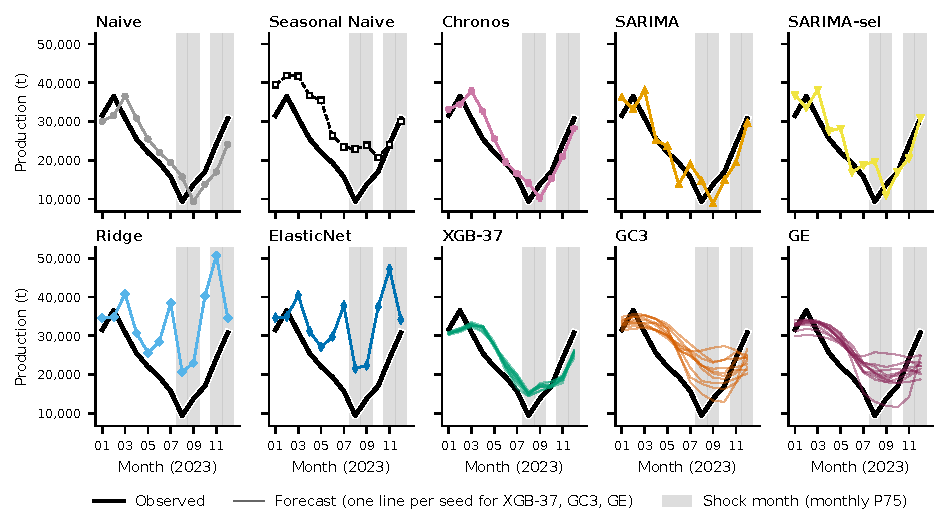
\includegraphics[width=\linewidth,height=0.36\textheight,keepaspectratio]{fig20_real_vs_pred_2023_sutil.pdf}
\caption{Sour lime, 2023}
\label{fig:fig20_real_vs_pred_2023_sutil}
\end{subfigure}
\par\medskip
\begin{subfigure}{\linewidth}
\centering
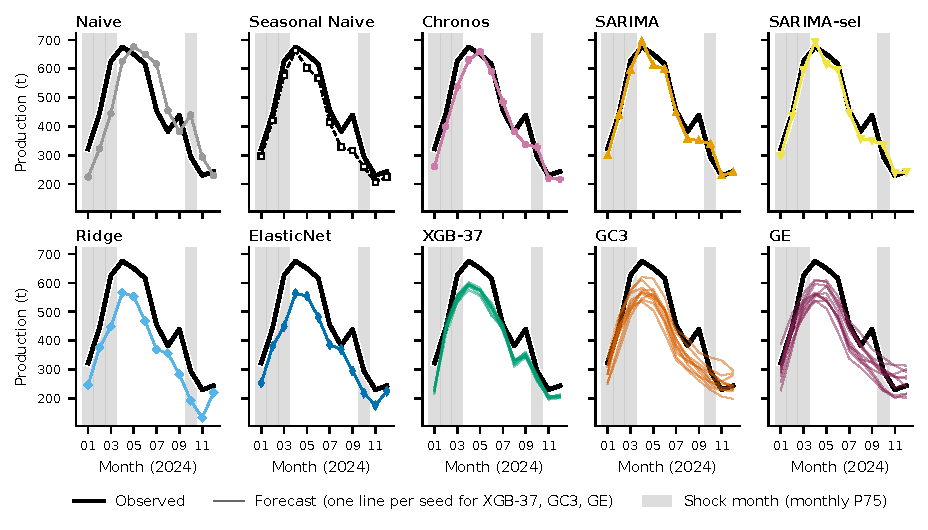
\includegraphics[width=\linewidth,height=0.36\textheight,keepaspectratio]{fig20_real_vs_pred_2024_dulce.pdf}
\caption{Sweet lime, 2024}
\label{fig:fig20_real_vs_pred_2024_dulce}
\end{subfigure}
\caption{\textit{Sour lime, 2023:} \figcap{fig20_real_vs_pred_2023_sutil} \textit{Sweet lime, 2024:} \figcap{fig20_real_vs_pred_2024_dulce}}
\label{fig:fig20_real_vs_pred_2023_sutil__fig20_real_vs_pred_2024_dulce}
\end{figure}

\begin{figure}[htbp]
\centering
\begin{subfigure}{\linewidth}
\centering
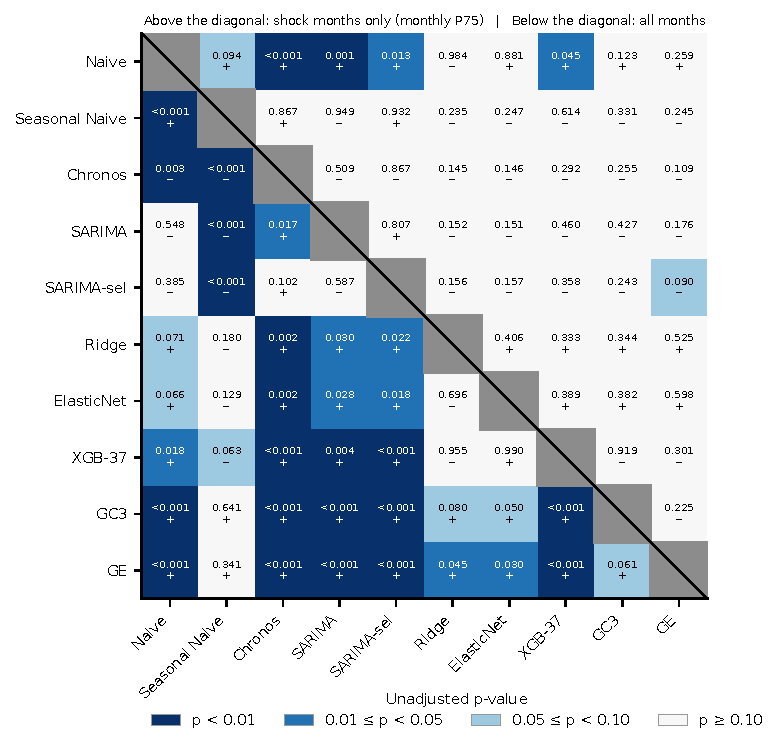
\includegraphics[width=\linewidth,height=0.36\textheight,keepaspectratio]{fig19_dm_pvalue_matrix_sutil.pdf}
\caption{Sour lime}
\label{fig:fig19_dm_pvalue_matrix_sutil}
\end{subfigure}
\par\medskip
\begin{subfigure}{\linewidth}
\centering
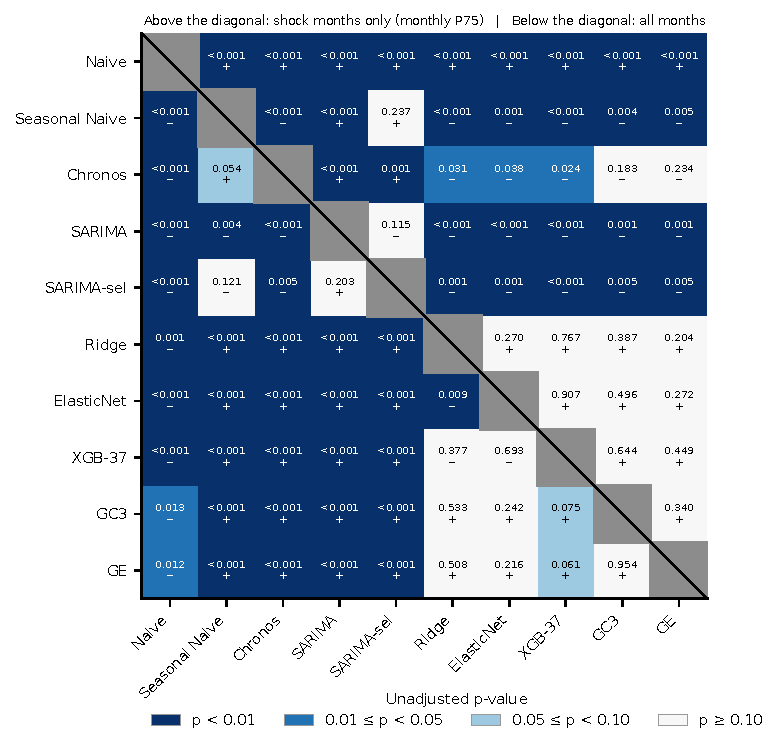
\includegraphics[width=\linewidth,height=0.36\textheight,keepaspectratio]{fig19_dm_pvalue_matrix_dulce.pdf}
\caption{Sweet lime}
\label{fig:fig19_dm_pvalue_matrix_dulce}
\end{subfigure}
\caption{\textit{Sour lime:} \figcap{fig19_dm_pvalue_matrix_sutil} \textit{Sweet lime:} \figcap{fig19_dm_pvalue_matrix_dulce}}
\label{fig:fig19_dm_pvalue_matrix}
\end{figure}

\begin{figure}[htbp]
\centering
\begin{subfigure}{\linewidth}
\centering
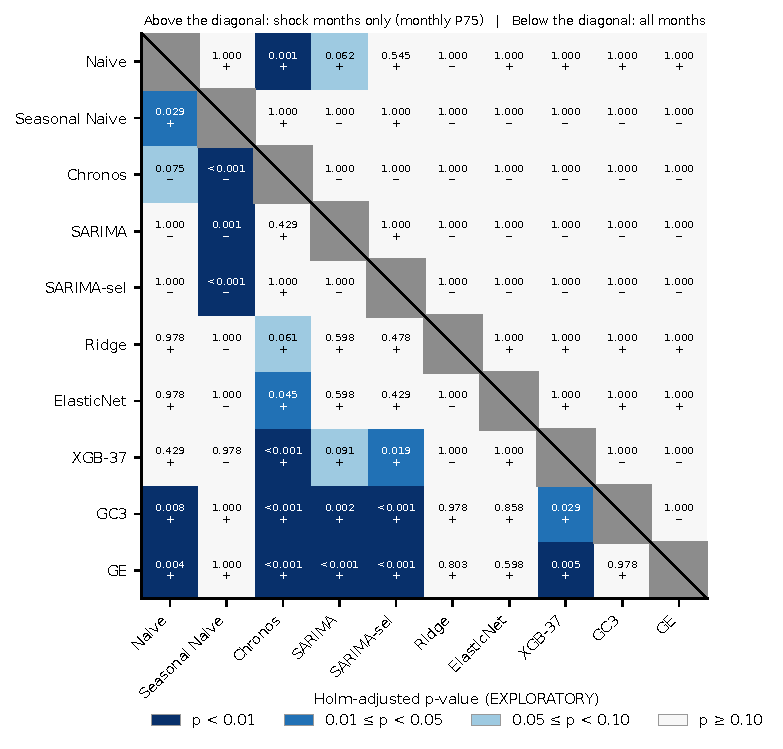
\includegraphics[width=\linewidth,height=0.36\textheight,keepaspectratio]{fig19b_dm_pvalue_matrix_holm_sutil.pdf}
\caption{Sour lime}
\label{fig:fig19b_dm_pvalue_matrix_holm_sutil}
\end{subfigure}
\par\medskip
\begin{subfigure}{\linewidth}
\centering
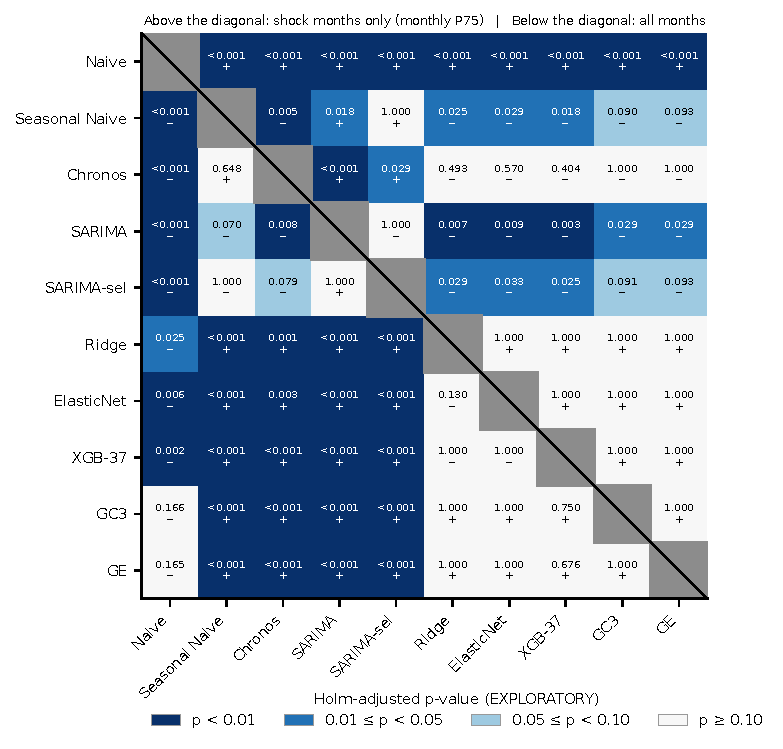
\includegraphics[width=\linewidth,height=0.36\textheight,keepaspectratio]{fig19b_dm_pvalue_matrix_holm_dulce.pdf}
\caption{Sweet lime}
\label{fig:fig19b_dm_pvalue_matrix_holm_dulce}
\end{subfigure}
\caption{\textbf{EXPLORATORY.} \textit{Sour lime:} \figcap{fig19b_dm_pvalue_matrix_holm_sutil} \textit{Sweet lime:} \figcap{fig19b_dm_pvalue_matrix_holm_dulce}}
\label{fig:fig19b_dm_pvalue_matrix_holm}
\end{figure}

\begin{figure}[htbp]
\centering
\begin{subfigure}{\linewidth}
\centering
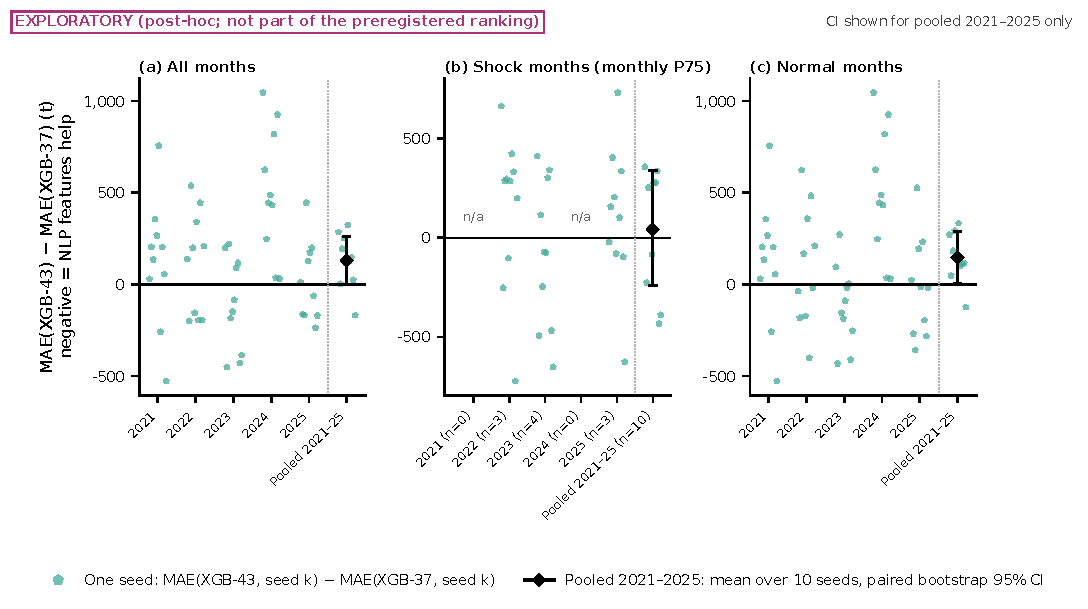
\includegraphics[width=\linewidth,height=0.36\textheight,keepaspectratio]{fig18b_xgb43_vs_xgb37_exploratory_sutil.pdf}
\caption{Sour lime}
\label{fig:fig18b_xgb43_vs_xgb37_exploratory_sutil}
\end{subfigure}
\par\medskip
\begin{subfigure}{\linewidth}
\centering
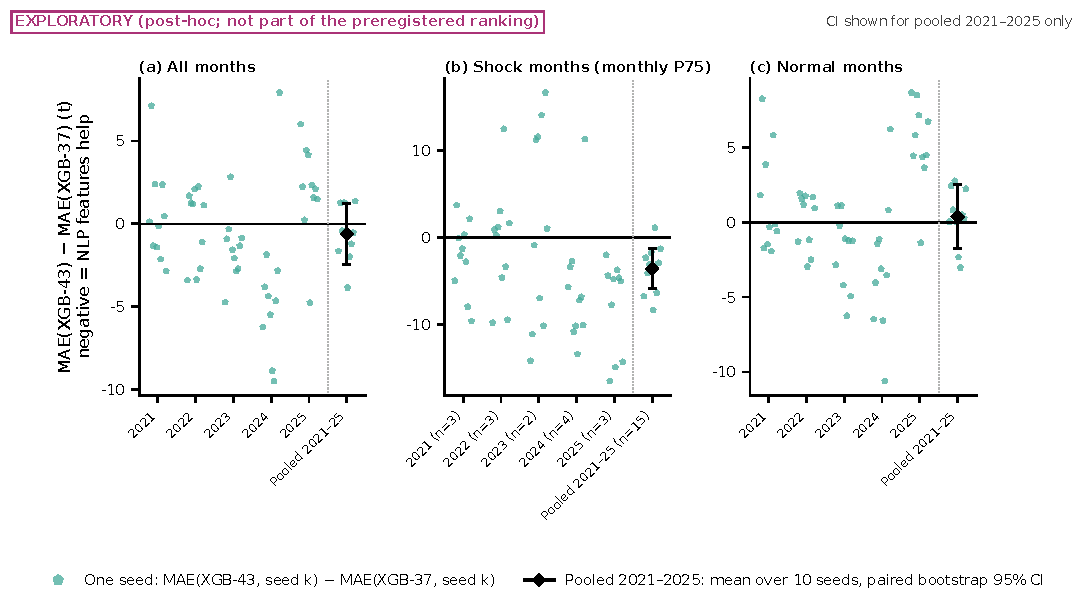
\includegraphics[width=\linewidth,height=0.36\textheight,keepaspectratio]{fig18b_xgb43_vs_xgb37_exploratory_dulce.pdf}
\caption{Sweet lime}
\label{fig:fig18b_xgb43_vs_xgb37_exploratory_dulce}
\end{subfigure}
\caption{\textit{Sour lime:} \figcap{fig18b_xgb43_vs_xgb37_exploratory_sutil} \textit{Sweet lime:} \figcap{fig18b_xgb43_vs_xgb37_exploratory_dulce}}
\label{fig:fig18b_xgb43_vs_xgb37_exploratory}
\end{figure}

\begin{figure}[htbp]
\centering
\begin{subfigure}{\linewidth}
\centering
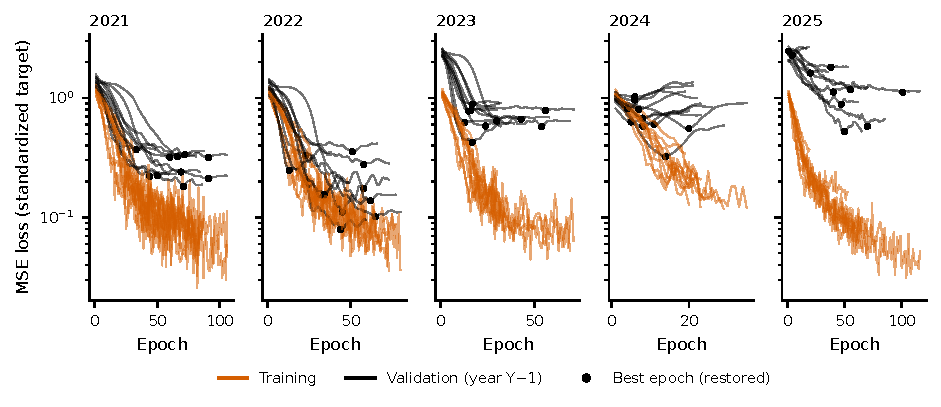
\includegraphics[width=\linewidth,height=0.36\textheight,keepaspectratio]{fig01_loss_curves_gc3_sutil.pdf}
\caption{Sour lime}
\label{fig:fig01_loss_curves_gc3_sutil}
\end{subfigure}
\par\medskip
\begin{subfigure}{\linewidth}
\centering
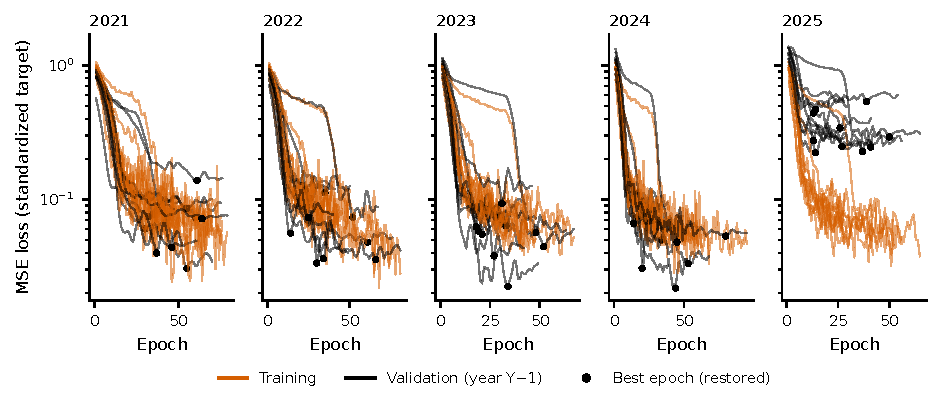
\includegraphics[width=\linewidth,height=0.36\textheight,keepaspectratio]{fig01_loss_curves_gc3_dulce.pdf}
\caption{Sweet lime}
\label{fig:fig01_loss_curves_gc3_dulce}
\end{subfigure}
\caption{\textit{Sour lime:} \figcap{fig01_loss_curves_gc3_sutil} \textit{Sweet lime:} \figcap{fig01_loss_curves_gc3_dulce}}
\label{fig:fig01_loss_curves_gc3}
\end{figure}

\begin{figure}[htbp]
\centering
\begin{subfigure}{\linewidth}
\centering
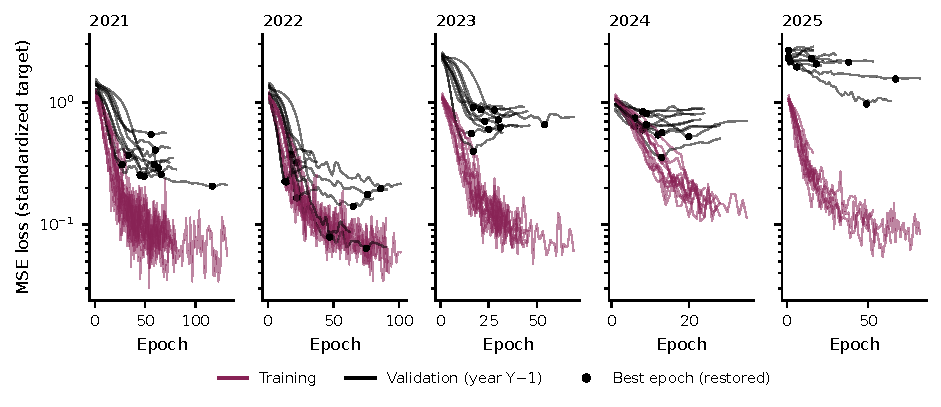
\includegraphics[width=\linewidth,height=0.36\textheight,keepaspectratio]{fig01_loss_curves_ge_sutil.pdf}
\caption{Sour lime}
\label{fig:fig01_loss_curves_ge_sutil}
\end{subfigure}
\par\medskip
\begin{subfigure}{\linewidth}
\centering
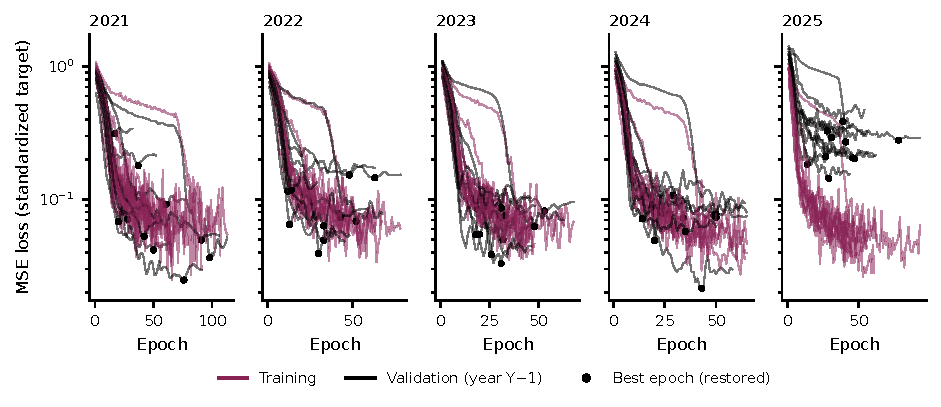
\includegraphics[width=\linewidth,height=0.36\textheight,keepaspectratio]{fig01_loss_curves_ge_dulce.pdf}
\caption{Sweet lime}
\label{fig:fig01_loss_curves_ge_dulce}
\end{subfigure}
\caption{\textit{Sour lime:} \figcap{fig01_loss_curves_ge_sutil} \textit{Sweet lime:} \figcap{fig01_loss_curves_ge_dulce}}
\label{fig:fig01_loss_curves_ge}
\end{figure}

\begin{figure}[htbp]
\centering
\begin{subfigure}{\linewidth}
\centering
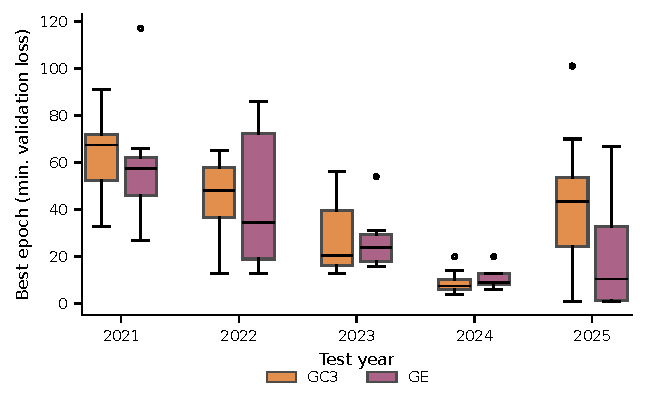
\includegraphics[width=\linewidth,height=0.36\textheight,keepaspectratio]{fig03_early_stopping_epoch_sutil.pdf}
\caption{Sour lime}
\label{fig:fig03_early_stopping_epoch_sutil}
\end{subfigure}
\par\medskip
\begin{subfigure}{\linewidth}
\centering
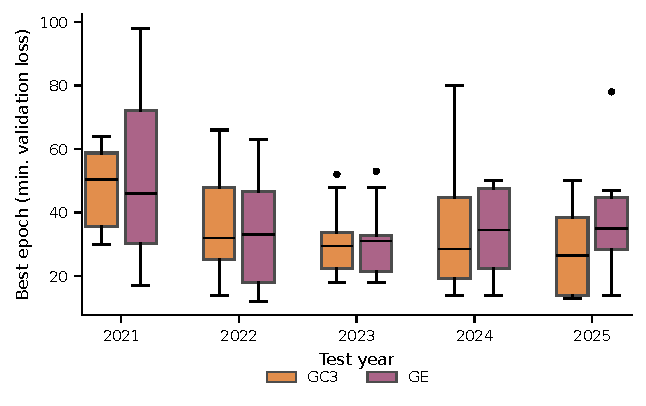
\includegraphics[width=\linewidth,height=0.36\textheight,keepaspectratio]{fig03_early_stopping_epoch_dulce.pdf}
\caption{Sweet lime}
\label{fig:fig03_early_stopping_epoch_dulce}
\end{subfigure}
\caption{\textit{Sour lime:} \figcap{fig03_early_stopping_epoch_sutil} \textit{Sweet lime:} \figcap{fig03_early_stopping_epoch_dulce}}
\label{fig:fig03_early_stopping_epoch}
\end{figure}

\begin{figure}[htbp]
\centering
\begin{subfigure}{\linewidth}
\centering
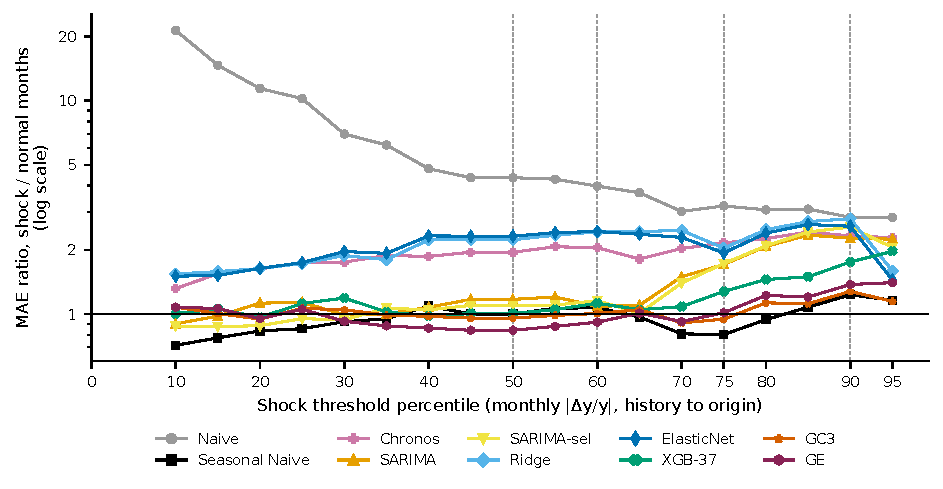
\includegraphics[width=\linewidth,height=0.36\textheight,keepaspectratio]{fig06_ratio_shock_normal_vs_percentile_sutil.pdf}
\caption{Sour lime}
\label{fig:fig06_ratio_shock_normal_vs_percentile_sutil}
\end{subfigure}
\par\medskip
\begin{subfigure}{\linewidth}
\centering
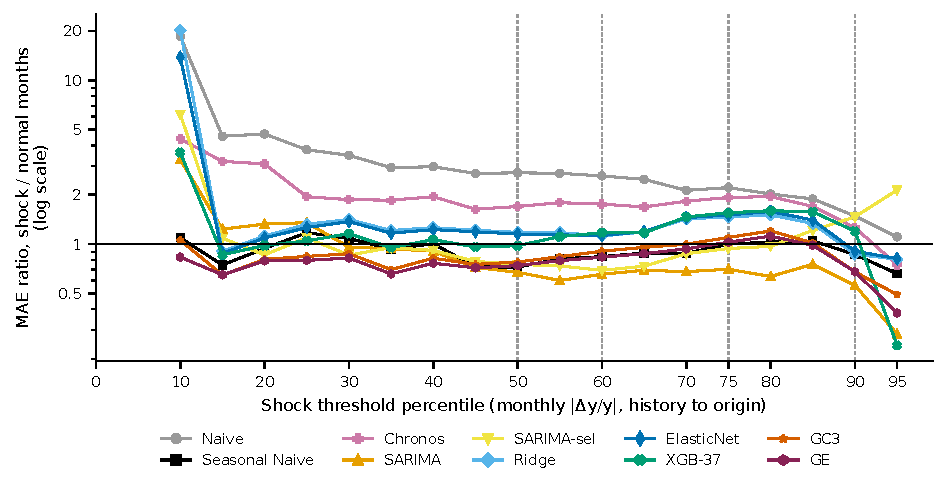
\includegraphics[width=\linewidth,height=0.36\textheight,keepaspectratio]{fig06_ratio_shock_normal_vs_percentile_dulce.pdf}
\caption{Sweet lime}
\label{fig:fig06_ratio_shock_normal_vs_percentile_dulce}
\end{subfigure}
\caption{\textit{Sour lime:} \figcap{fig06_ratio_shock_normal_vs_percentile_sutil} \textit{Sweet lime:} \figcap{fig06_ratio_shock_normal_vs_percentile_dulce}}
\label{fig:fig06_ratio_shock_normal_vs_percentile}
\end{figure}

\begin{figure}[htbp]
\centering
\begin{subfigure}{\linewidth}
\centering
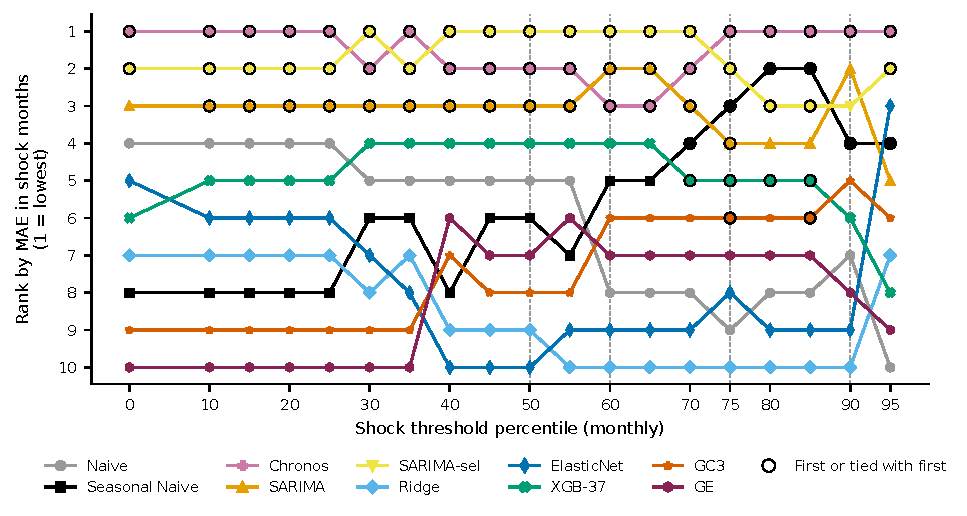
\includegraphics[width=\linewidth,height=0.36\textheight,keepaspectratio]{fig08_rank_bump_chart_sutil.pdf}
\caption{Sour lime}
\label{fig:fig08_rank_bump_chart_sutil}
\end{subfigure}
\par\medskip
\begin{subfigure}{\linewidth}
\centering
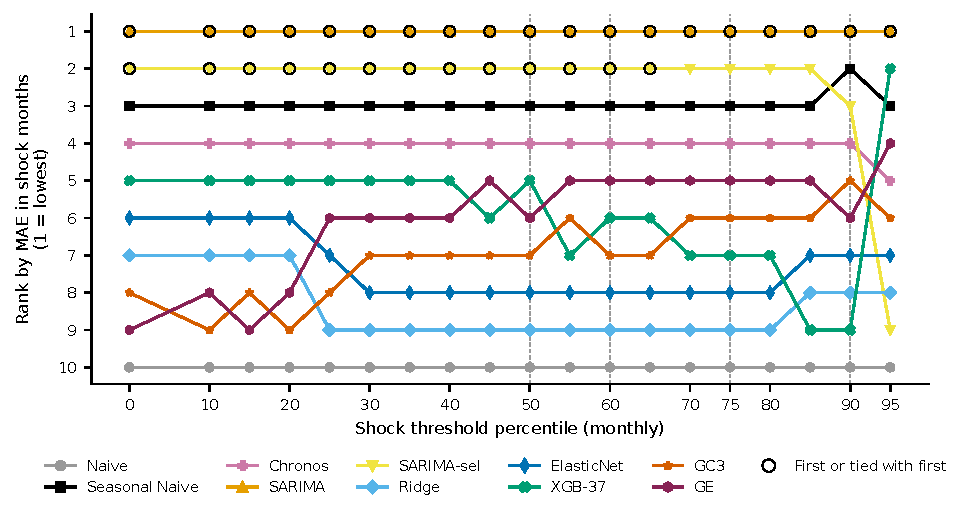
\includegraphics[width=\linewidth,height=0.36\textheight,keepaspectratio]{fig08_rank_bump_chart_dulce.pdf}
\caption{Sweet lime}
\label{fig:fig08_rank_bump_chart_dulce}
\end{subfigure}
\caption{\textit{Sour lime:} \figcap{fig08_rank_bump_chart_sutil} \textit{Sweet lime:} \figcap{fig08_rank_bump_chart_dulce}}
\label{fig:fig08_rank_bump_chart}
\end{figure}

\begin{figure}[htbp]
\centering
\begin{subfigure}{0.49\linewidth}
\centering
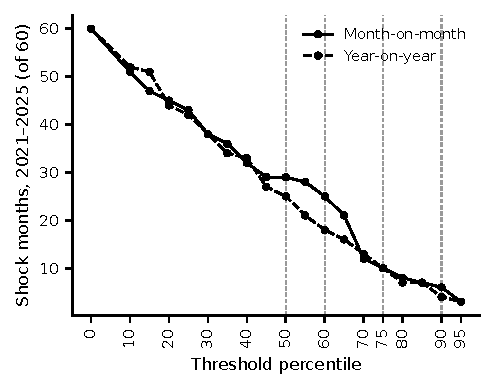
\includegraphics[width=\linewidth]{fig09_n_shock_vs_percentile_sutil.pdf}
\caption{Sour lime}
\label{fig:fig09_n_shock_vs_percentile_sutil}
\end{subfigure}\hfill
\begin{subfigure}{0.49\linewidth}
\centering
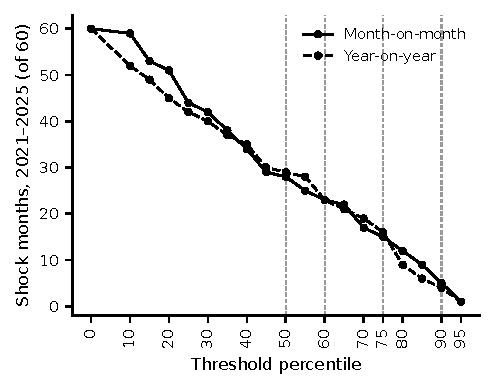
\includegraphics[width=\linewidth]{fig09_n_shock_vs_percentile_dulce.pdf}
\caption{Sweet lime}
\label{fig:fig09_n_shock_vs_percentile_dulce}
\end{subfigure}
\caption{\textit{Sour lime:} \figcap{fig09_n_shock_vs_percentile_sutil} \textit{Sweet lime:} \figcap{fig09_n_shock_vs_percentile_dulce}}
\label{fig:fig09_n_shock_vs_percentile}
\end{figure}

\begin{figure}[htbp]
\centering
\begin{subfigure}{\linewidth}
\centering
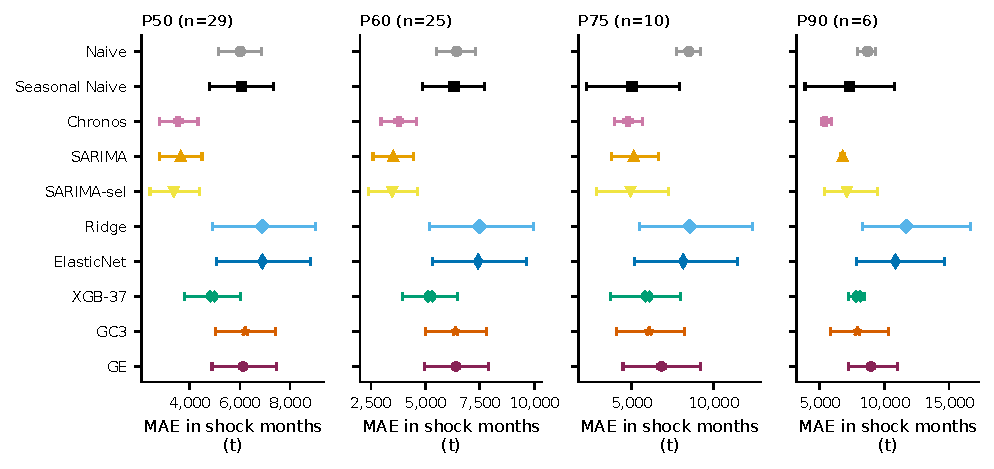
\includegraphics[width=\linewidth,height=0.36\textheight,keepaspectratio]{fig11_bootstrap_ci_mae_shock_report_points_sutil.pdf}
\caption{Sour lime}
\label{fig:fig11_bootstrap_ci_mae_shock_report_points_sutil}
\end{subfigure}
\par\medskip
\begin{subfigure}{\linewidth}
\centering
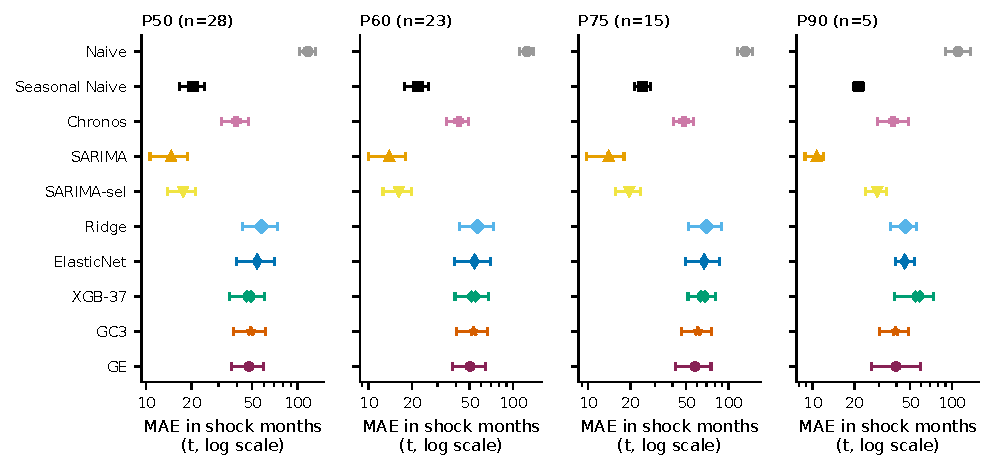
\includegraphics[width=\linewidth,height=0.36\textheight,keepaspectratio]{fig11_bootstrap_ci_mae_shock_report_points_dulce.pdf}
\caption{Sweet lime}
\label{fig:fig11_bootstrap_ci_mae_shock_report_points_dulce}
\end{subfigure}
\caption{\textit{Sour lime:} \figcap{fig11_bootstrap_ci_mae_shock_report_points_sutil} \textit{Sweet lime:} \figcap{fig11_bootstrap_ci_mae_shock_report_points_dulce}}
\label{fig:fig11_bootstrap_ci_mae_shock_report_points}
\end{figure}

\begin{figure}[htbp]
\centering
\begin{subfigure}{\linewidth}
\centering
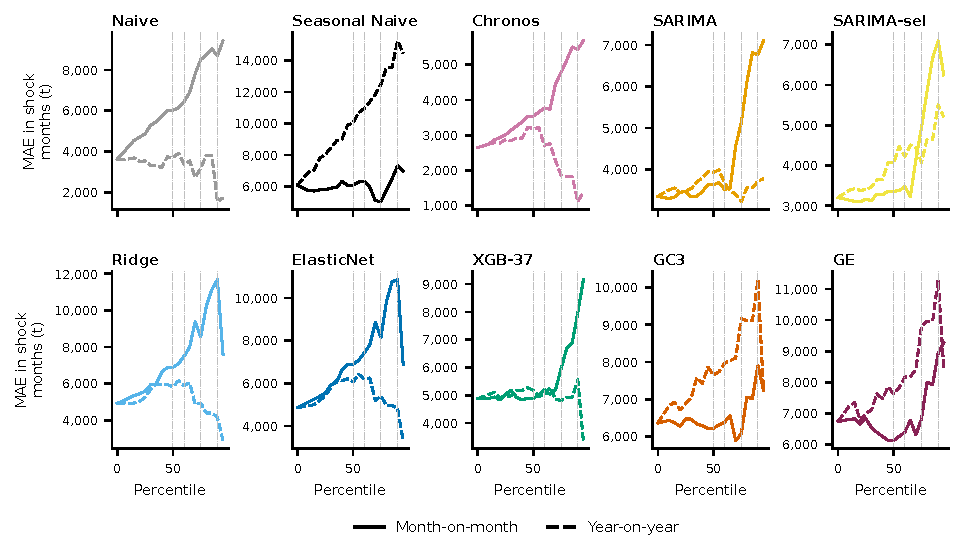
\includegraphics[width=\linewidth,height=0.36\textheight,keepaspectratio]{fig12_yoy_vs_mom_threshold_sutil.pdf}
\caption{Sour lime}
\label{fig:fig12_yoy_vs_mom_threshold_sutil}
\end{subfigure}
\par\medskip
\begin{subfigure}{\linewidth}
\centering
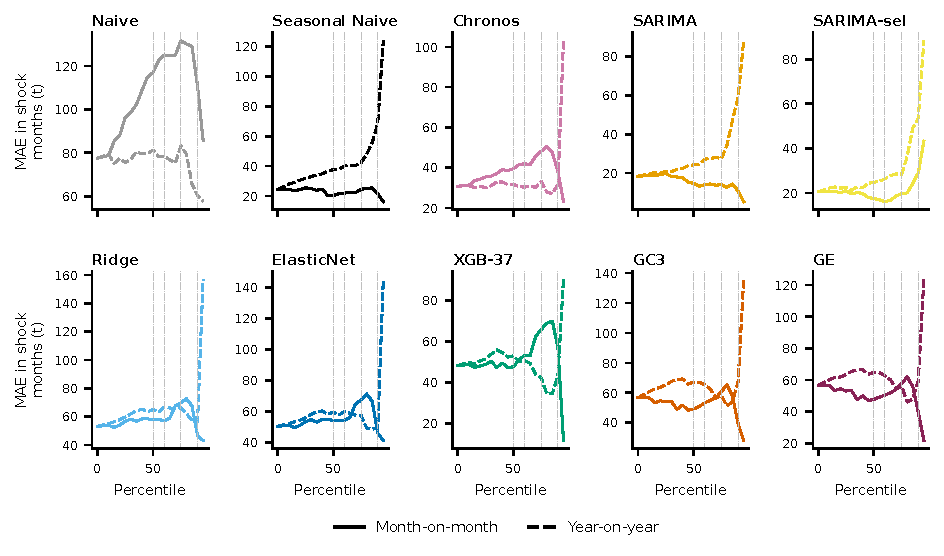
\includegraphics[width=\linewidth,height=0.36\textheight,keepaspectratio]{fig12_yoy_vs_mom_threshold_dulce.pdf}
\caption{Sweet lime}
\label{fig:fig12_yoy_vs_mom_threshold_dulce}
\end{subfigure}
\caption{\textit{Sour lime:} \figcap{fig12_yoy_vs_mom_threshold_sutil} \textit{Sweet lime:} \figcap{fig12_yoy_vs_mom_threshold_dulce}}
\label{fig:fig12_yoy_vs_mom_threshold}
\end{figure}

\begin{figure}[htbp]
\centering
\begin{subfigure}{\linewidth}
\centering
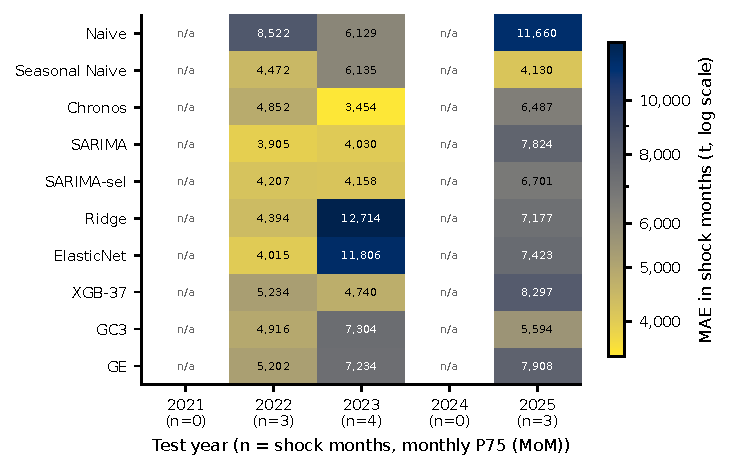
\includegraphics[width=\linewidth,height=0.36\textheight,keepaspectratio]{fig14_mae_shock_heatmap_model_window_sutil.pdf}
\caption{Sour lime}
\label{fig:fig14_mae_shock_heatmap_model_window_sutil}
\end{subfigure}
\par\medskip
\begin{subfigure}{\linewidth}
\centering
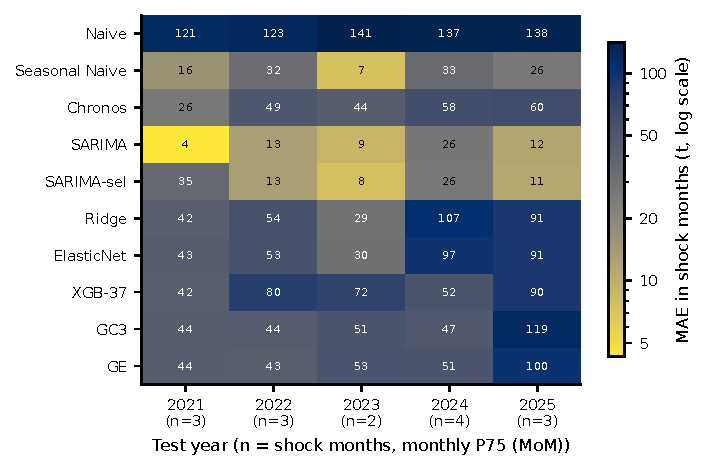
\includegraphics[width=\linewidth,height=0.36\textheight,keepaspectratio]{fig14_mae_shock_heatmap_model_window_dulce.pdf}
\caption{Sweet lime}
\label{fig:fig14_mae_shock_heatmap_model_window_dulce}
\end{subfigure}
\caption{\textit{Sour lime:} \figcap{fig14_mae_shock_heatmap_model_window_sutil} \textit{Sweet lime:} \figcap{fig14_mae_shock_heatmap_model_window_dulce}}
\label{fig:fig14_mae_shock_heatmap_model_window}
\end{figure}

\begin{figure}[htbp]
\centering
\begin{subfigure}{\linewidth}
\centering
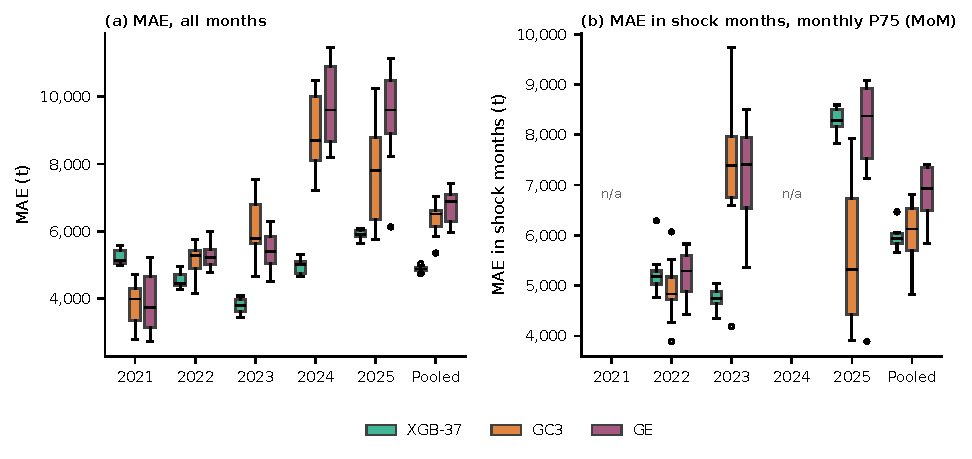
\includegraphics[width=\linewidth,height=0.36\textheight,keepaspectratio]{fig15_seed_boxplots_sutil.pdf}
\caption{Sour lime}
\label{fig:fig15_seed_boxplots_sutil}
\end{subfigure}
\par\medskip
\begin{subfigure}{\linewidth}
\centering
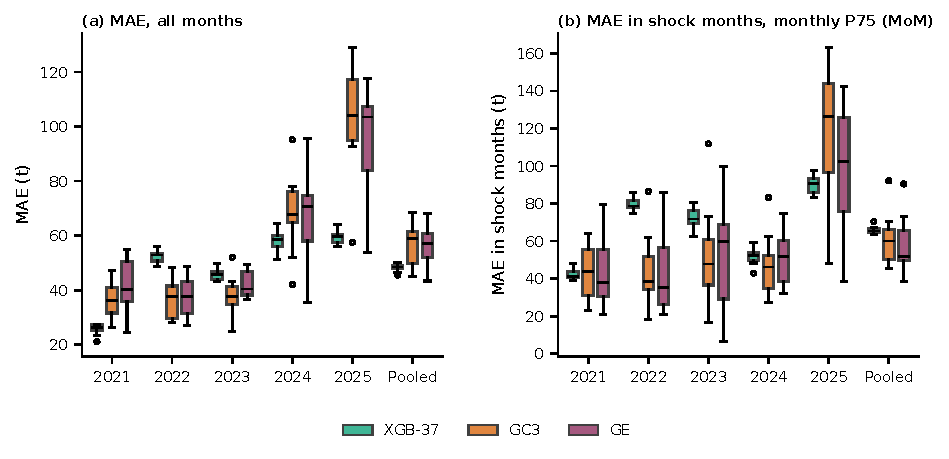
\includegraphics[width=\linewidth,height=0.36\textheight,keepaspectratio]{fig15_seed_boxplots_dulce.pdf}
\caption{Sweet lime}
\label{fig:fig15_seed_boxplots_dulce}
\end{subfigure}
\caption{\textit{Sour lime:} \figcap{fig15_seed_boxplots_sutil} \textit{Sweet lime:} \figcap{fig15_seed_boxplots_dulce}}
\label{fig:fig15_seed_boxplots}
\end{figure}

\begin{figure}[htbp]
\centering
\begin{subfigure}{\linewidth}
\centering
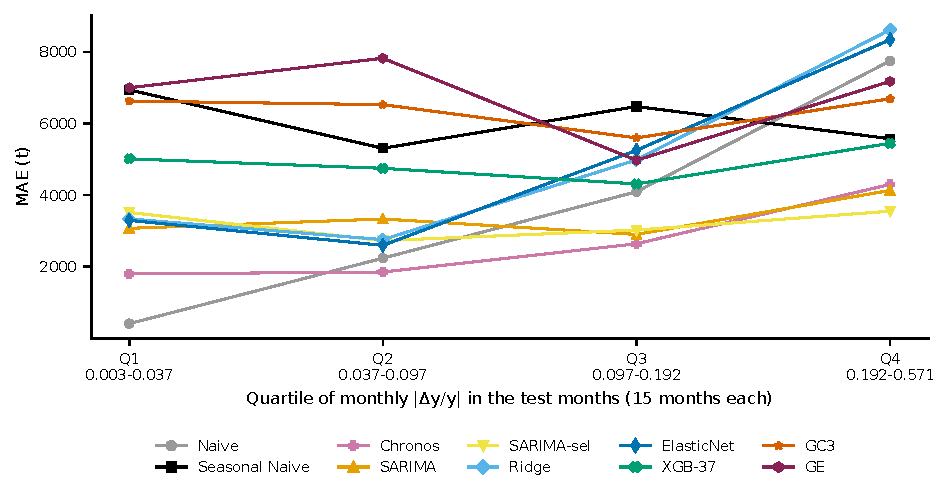
\includegraphics[width=\linewidth,height=0.36\textheight,keepaspectratio]{fig16_mae_by_change_quartile_sutil.pdf}
\caption{Sour lime}
\label{fig:fig16_mae_by_change_quartile_sutil}
\end{subfigure}
\par\medskip
\begin{subfigure}{\linewidth}
\centering
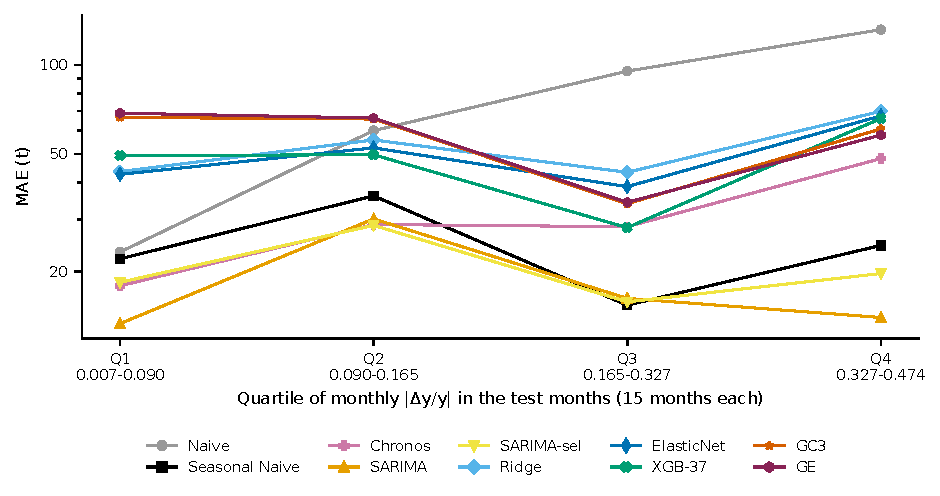
\includegraphics[width=\linewidth,height=0.36\textheight,keepaspectratio]{fig16_mae_by_change_quartile_dulce.pdf}
\caption{Sweet lime}
\label{fig:fig16_mae_by_change_quartile_dulce}
\end{subfigure}
\caption{\textit{Sour lime:} \figcap{fig16_mae_by_change_quartile_sutil} \textit{Sweet lime:} \figcap{fig16_mae_by_change_quartile_dulce}}
\label{fig:fig16_mae_by_change_quartile}
\end{figure}

\begin{figure}[htbp]
\centering
\begin{subfigure}{\linewidth}
\centering
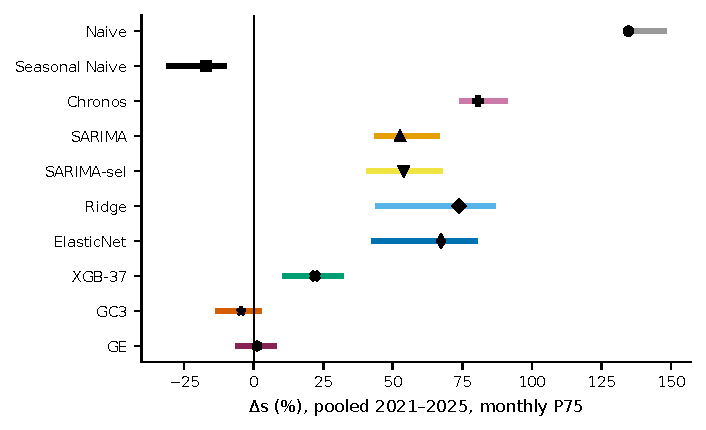
\includegraphics[width=\linewidth,height=0.36\textheight,keepaspectratio]{fig17_leave_one_shock_out_delta_s_sutil.pdf}
\caption{Sour lime}
\label{fig:fig17_leave_one_shock_out_delta_s_sutil}
\end{subfigure}
\par\medskip
\begin{subfigure}{\linewidth}
\centering
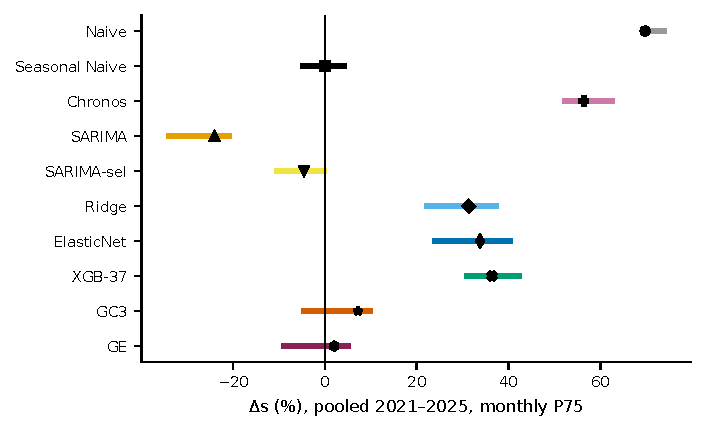
\includegraphics[width=\linewidth,height=0.36\textheight,keepaspectratio]{fig17_leave_one_shock_out_delta_s_dulce.pdf}
\caption{Sweet lime}
\label{fig:fig17_leave_one_shock_out_delta_s_dulce}
\end{subfigure}
\caption{\textit{Sour lime:} \figcap{fig17_leave_one_shock_out_delta_s_sutil} \textit{Sweet lime:} \figcap{fig17_leave_one_shock_out_delta_s_dulce}}
\label{fig:fig17_leave_one_shock_out_delta_s}
\end{figure}

\begin{figure}[htbp]
\centering
\begin{subfigure}{\linewidth}
\centering
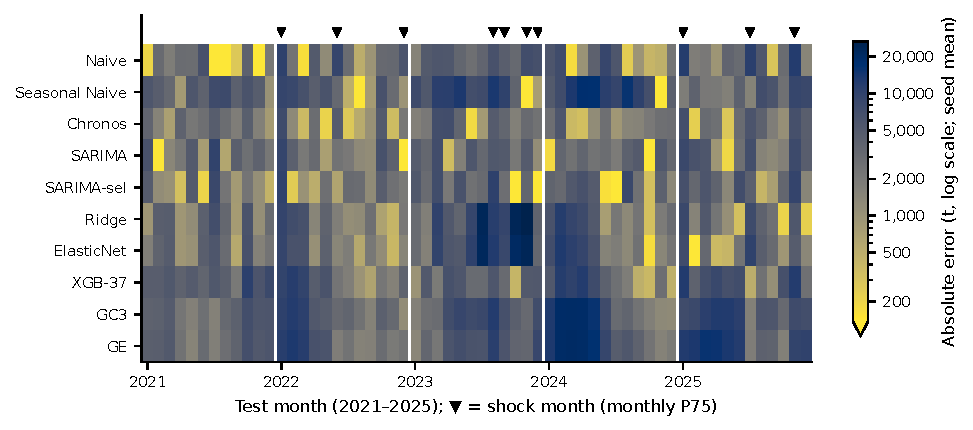
\includegraphics[width=\linewidth,height=0.36\textheight,keepaspectratio]{fig21_abs_error_monthly_sutil.pdf}
\caption{Sour lime}
\label{fig:fig21_abs_error_monthly_sutil}
\end{subfigure}
\par\medskip
\begin{subfigure}{\linewidth}
\centering
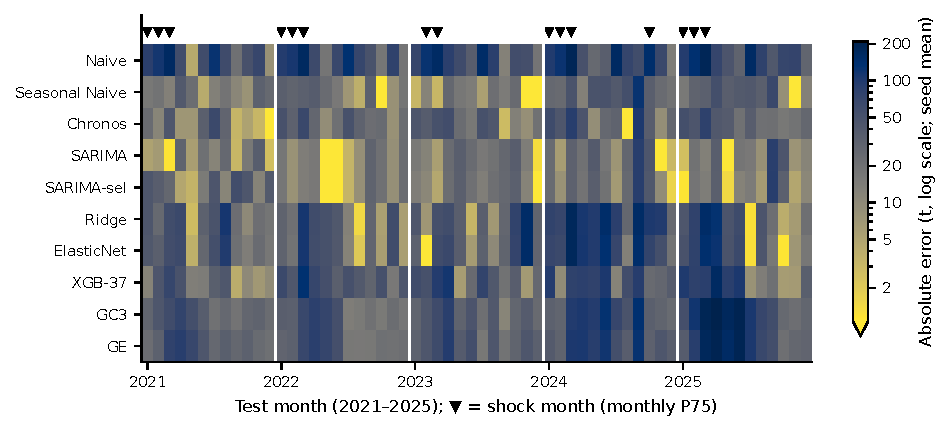
\includegraphics[width=\linewidth,height=0.36\textheight,keepaspectratio]{fig21_abs_error_monthly_dulce.pdf}
\caption{Sweet lime}
\label{fig:fig21_abs_error_monthly_dulce}
\end{subfigure}
\caption{\textit{Sour lime:} \figcap{fig21_abs_error_monthly_sutil} \textit{Sweet lime:} \figcap{fig21_abs_error_monthly_dulce}}
\label{fig:fig21_abs_error_monthly}
\end{figure}
